% This is the Reed College LaTeX thesis template. Most of the work
% for the document class was done by Sam Noble (SN), as well as this
% template. Later comments etc. by Ben Salzberg (BTS). Additional
% restructuring and APA support by Jess Youngberg (JY).
% Your comments and suggestions are more than welcome; please email
% them to cus@reed.edu
%
% See https://www.reed.edu/cis/help/LaTeX/index.html for help. There are a
% great bunch of help pages there, with notes on
% getting started, bibtex, etc. Go there and read it if you're not
% already familiar with LaTeX.
%
% Any line that starts with a percent symbol is a comment.
% They won't show up in the document, and are useful for notes
% to yourself and explaining commands.
% Commenting also removes a line from the document;
% very handy for troubleshooting problems. -BTS

% As far as I know, this follows the requirements laid out in
% the 2002-2003 Senior Handbook. Ask a librarian to check the
% document before binding. -SN

%%
%% Preamble
%%
% \documentclass{<something>} must begin each LaTeX document
\documentclass[12pt,twoside]{templates/facsothesis}
% Packages are extensions to the basic LaTeX functions. Whatever you
% want to typeset, there is probably a package out there for it.
% Chemistry (chemtex), screenplays, you name it.
% Check out CTAN to see: https://www.ctan.org/
%%
\ifxetex
  \usepackage{polyglossia}
  \setmainlanguage{spanish}
  % Tabla en lugar de cuadro
  \gappto\captionsspanish{\renewcommand{\tablename}{Tabla}
          \renewcommand{\listtablename}{Índice de tablas}}
\else
  \usepackage[spanish,es-tabla]{babel}
\fi
%\usepackage[spanish]{babel}
\usepackage{graphicx,latexsym}
\usepackage{amsmath}
\usepackage{amssymb,amsthm}
\usepackage{longtable,booktabs,setspace}
\usepackage{chemarr} %% Useful for one reaction arrow, useless if you're not a chem major
\usepackage[hyphens]{url}
% Added by CII
%\usepackage{hyperref}
\usepackage[colorlinks = true,
            linkcolor = blue,
            urlcolor  = blue,
            citecolor = blue,
            anchorcolor = blue]{hyperref}
\usepackage{lmodern}
\usepackage{float}
\floatplacement{figure}{H}
% End of CII addition
\usepackage{rotating}
\usepackage{placeins} % para fijar la posición de las tablas con \FloatBarrier


\usepackage[]{natbib}


% Next line commented out by CII
%\usepackage{biblatex}
%\usepackage{natbib}
% Comment out the natbib line above and uncomment the following two lines to use the new
% biblatex-chicago style, for Chicago A. Also make some changes at the end where the
% bibliography is included.
%\usepackage{biblatex-chicago}
%\bibliography{thesis}


% Added by CII (Thanks, Hadley!)
% Use ref for internal links
\renewcommand{\hyperref}[2][???]{\autoref{#1}}
\def\chapterautorefname{Chapter}
\def\sectionautorefname{Section}
\def\subsectionautorefname{Subsection}
% End of CII addition

% Added by CII
\usepackage{caption}
\captionsetup{width=5in}
% End of CII addition

% \usepackage{times} % other fonts are available like times, bookman, charter, palatino

% Syntax highlighting #22

% To pass between YAML and LaTeX the dollar signs are added by CII
\title{Aceptar la diversidad en el vecindario}
\author{Kevin Carrasco Quintanilla}
% The month and year that you submit your FINAL draft TO THE LIBRARY (May or December)
\date{2022-11-28}
\division{}
\advisor{Profesor guía: Juan Carlos Castillo}
\institution{Universidad de Chile}
\degree{Magister en ciencias sociales mención en sociología de la modernización}
%If you have two advisors for some reason, you can use the following
% Uncommented out by CII
% End of CII addition

%%% Remember to use the correct department!
\department{}
% if you're writing a thesis in an interdisciplinary major,
% uncomment the line below and change the text as appropriate.
% check the Senior Handbook if unsure.
%\thedivisionof{The Established Interdisciplinary Committee for}
% if you want the approval page to say "Approved for the Committee",
% uncomment the next line
%\approvedforthe{Committee}

% Added by CII
%%% Copied from knitr
%% maxwidth is the original width if it's less than linewidth
%% otherwise use linewidth (to make sure the graphics do not exceed the margin)
\makeatletter
\def\maxwidth{ %
  \ifdim\Gin@nat@width>\linewidth
    \linewidth
  \else
    \Gin@nat@width
  \fi
}
\makeatother

%Added by @MyKo101, code provided by @GerbrichFerdinands

\setlength\parindent{0pt}


% Added by CII

\providecommand{\tightlist}{%
  \setlength{\itemsep}{0pt}\setlength{\parskip}{0pt}}

\Acknowledgements{

}

\Dedication{

}

\Preface{

}

\Abstract{

}

	\usepackage{booktabs}
\usepackage{longtable}
\usepackage{array}
\usepackage{multirow}
\usepackage{wrapfig}
\usepackage{float}
\usepackage{colortbl}
\usepackage{pdflscape}
\usepackage{tabu}
\usepackage{threeparttable}
\usepackage{threeparttablex}
\usepackage[normalem]{ulem}
\usepackage{makecell}
\usepackage{xcolor}
% End of CII addition
%%
%% End Preamble
%%
%
\let\chaptername\relax
\begin{document}
\bibliographystyle{apalike}
% Everything below added by CII
  \maketitle

\frontmatter % this stuff will be roman-numbered
\pagestyle{empty} % this removes page numbers from the frontmatter



%  \hypersetup{linkcolor=black}
  \setcounter{tocdepth}{1}
  \setlength{\parskip}{0pt}
  \tableofcontents

\setlength\parskip{1em plus 0.1em minus 0.2em}

  \listoftables

  \listoffigures



\mainmatter % here the regular arabic numbering starts
\pagestyle{fancyplain} % turns page numbering back on

\hypertarget{resumen}{%
\chapter{Resumen}\label{resumen}}

Las investigaciones sobre diversidad social se han situado frecuentemente bajo el paradigma de la integración social, es decir, en la forma en que distintos grupos sociales poseen determinada posición dentro de la estructura social (ej. Young 2000; Wade 2000; Viveros Vigoya 2016). Al situarse bajo este paradigma, se han dejado de lado dos elementos fundamentales. Por un lado, se ha estudiado en menor medida el proceso de inclusión social en las escuelas (Blanco 2006) y la percepción que la población tiene sobre los demás grupos, en el sentido de si aceptan o rechazan a determinados grupos sociales que son distintos o que poseen otras posiciones en la estructura social. Por otro lado, tampoco se ha abordado completamente el proceso mediante el cual se aprenden o reproducen en la sociedad las actitudes de las personas en relación con estos grupos sociales.

Las escuelas en las sociedades democráticas suelen ser consideradas como responsables de transmitir conocimientos y habilidades, enfocadas en la comprensión de las estructuras y procesos sociales (Torney-Purta et. al 2008; Sandoval-Hernández, et. al 2018). Para la sociología, la comprensión de la educación como un agente de socialización de las generaciones más jóvenes resulta fundamental, donde específicamente los aprendizajes que se le adjudican a la educación ciudadana en las escuelas buscan dar respuesta a la necesidad de preparar a las nuevas generaciones para la vida en democracia y sus requerimientos morales y cognitivos (Cox y García 2015). Asimismo, dentro de la sociología el rol de la familia ha sido estudiado en menor medida, donde algunas investigaciones han dado cuenta del efecto de las actitudes de los padres en el conflicto interétnico de su descendencia (Medjedovic y Petrovic 2021) y que las familias de clase alta tienden a privilegiar valores más simbólico-relacionales, como los buenos modales y el respeto por los demás, mientras que las clases bajas privilegiarían transmitir valores de ascenso social, como el trabajo duro y el ahorro (Santander, et. al 2020). Finalmente, también se ha demostrado que ciertos patrones de segregación territorial influyen en la percepción y la confianza entre grupos distintos (Baldassarri y Abascal 2020; Fernández, et. al 2016; Coté y Erickson 2009).

De esta forma, esta investigación pretende abordar estas tres problemáticas en su conjunto, es decir, se pretende abordar si jóvenes en edad escolar aceptan o rechazan a diferentes grupos sociales y los distintos procesos de socialización que están implicados en el aprendizaje de estas actitudes. Específicamente, mediante metodologías cuantitativas se espera demostrar, por un lado, que la familia y la escuela influyen en el proceso de aprendizaje de actitudes, donde además se espera que la escuela logre disminuir las desigualdades de origen. Por otro lado, se espera demostrar que ciertas características contextuales de los territorios influyen en la aceptación o rechazo de distintos grupos sociales.

Los datos por utilizar provienen del primer estudio de Formación Ciudadana de Chile en 2017. Se cuenta con las respuestas de 8701 estudiantes y 6770 apoderados, provenientes de 242 escuelas del país.

\hypertarget{introducciuxf3n}{%
\chapter{Introducción:}\label{introducciuxf3n}}

Las nuevas dinámicas de migración, conflicto interétnico, diferencias de clase socioeconómica y segregación son de manera creciente puestas en confrontación en el debate público y cada vez más estudiadas por las Ciencias Sociales. Hasta ahora, las investigaciones en Sociología se han situado frecuentemente bajo el paradigma de la integración y exclusión social, es decir, en la forma en que distintos grupos sociales poseen determinada posición dentro de la estructura social \citep[ej.][]{young_justicia_2000, wade_raza_2000, viverosvigoya_interseccionalidad_2016}. Al situarse bajo este paradigma, se han dejado de lado dos elementos fundamentales. Por un lado, se ha estudiado en menor medida el proceso de inclusión social en las escuelas \citep{blanco_equidad_2006} y la percepción que la población tiene sobre los demás grupos al relacionarse con ellos en su vida cotidiana, en el sentido de si aceptan o rechazan a determinados grupos sociales que son distintos o que poseen otras posiciones en la estructura social. Por otro lado, ha ido cobrando reciente relevancia el proceso mediante el cual se aprenden o reproducen las actitudes de las personas en relación con la aceptación o rechazo de determinados grupos sociales y la importancia de la escuela en este proceso \citep{sandoval-hernandez_teaching_2018, malak-minkiewicz_influences_2021}. De esta forma, esta investigación pretende abordar estas dos problemáticas en su conjunto, es decir, se pretende abordar si jóvenes en edad escolar aceptan o rechazan a diferentes grupos sociales y los distintos procesos de socialización que están implicados en el aprendizaje de estas actitudes.

Los procesos de modernización y globalización en Chile y Latinoamérica han planteado distintos desafíos para lograr sus objetivos y por los resultados adversos que de ellos provienen. Según \citet{sunkel_sostenibilidad_1998}, el Siglo XXI comienza bajo una lógica de Apartheid, donde se crea un fenómeno de polarización en el que, por un lado, se genera un mejoramiento de la vida de segmentos muy limitados de la sociedad al tener una economía que crea muy poco empleo y, por otro lado, se genera exclusión social en segmentos crecientes de la población. Esta lógica dual también es retomada por \citet{castells_globalizacion_2005} al plantear que como la globalización es un instrumento de articulación de mercados capitalistas, la rentabilidad económica se convierte en el criterio fundamental para la inclusión o exclusión en las redes globales (donde se articulan o excluyen a ciertos individuos, grupos, países, regiones, etc.). En resumen, es el mismo proceso de globalización el que provoca y/o agrava los procesos de descomposición social \citep{lechner_debate_1992}.

Siguiendo el panorama mundial, con el aumento sostenido del desarrollo económico de los últimos años, se ha pasado de demandas sociales que apuntan a valores de supervivencia (demandas socioeconómicas, derechos sociales, acceso a servicios básicos, etc.) hacia demandas de auto expresión, creatividad y democratización que ayudan a remodelar las normas sexuales, los roles de género, los valores familiares, la religiosidad, la relación de las personas con la naturaleza y sus actividades comunitarias \citep{inglehart_Modernization_2001}, como tal, se han planteado importantes desafíos en términos de Democracia y Ciudadanía. En una investigación internacional de 21 países con datos de la Encuesta Mundial de Valores, \citet{vala_youth_2010} demuestra que los jóvenes son más tolerantes que las personas mayores hacia los grupos estigmatizados y los grupos percibidos como racial o étnicamente diferentes. En general durante los últimos años las actitudes de la población adulta en Chile han presentado un alza en el porcentaje de personas que aceptan que diferentes grupos sociales vivan en sus vecindarios. Los datos de la Encuesta Mundial de Valores \citep{haerpfer_world_2021} muestran en el Gráfico \ref{fig:aceptacion-wvs} que la aceptación a que grupos de distinta raza, distinta nacionalidad y de distinta orientación sexual vivan en sus vecindarios ha aumentado entre 1990 y 2018, exceptuando una pequeña variación en el último año para las personas de distinta nacionalidad. En el caso de las personas de distinta religión, el porcentaje de personas que las aceptan ha disminuido entre 2006 y 2018.

\begin{figure}[H]

{\centering 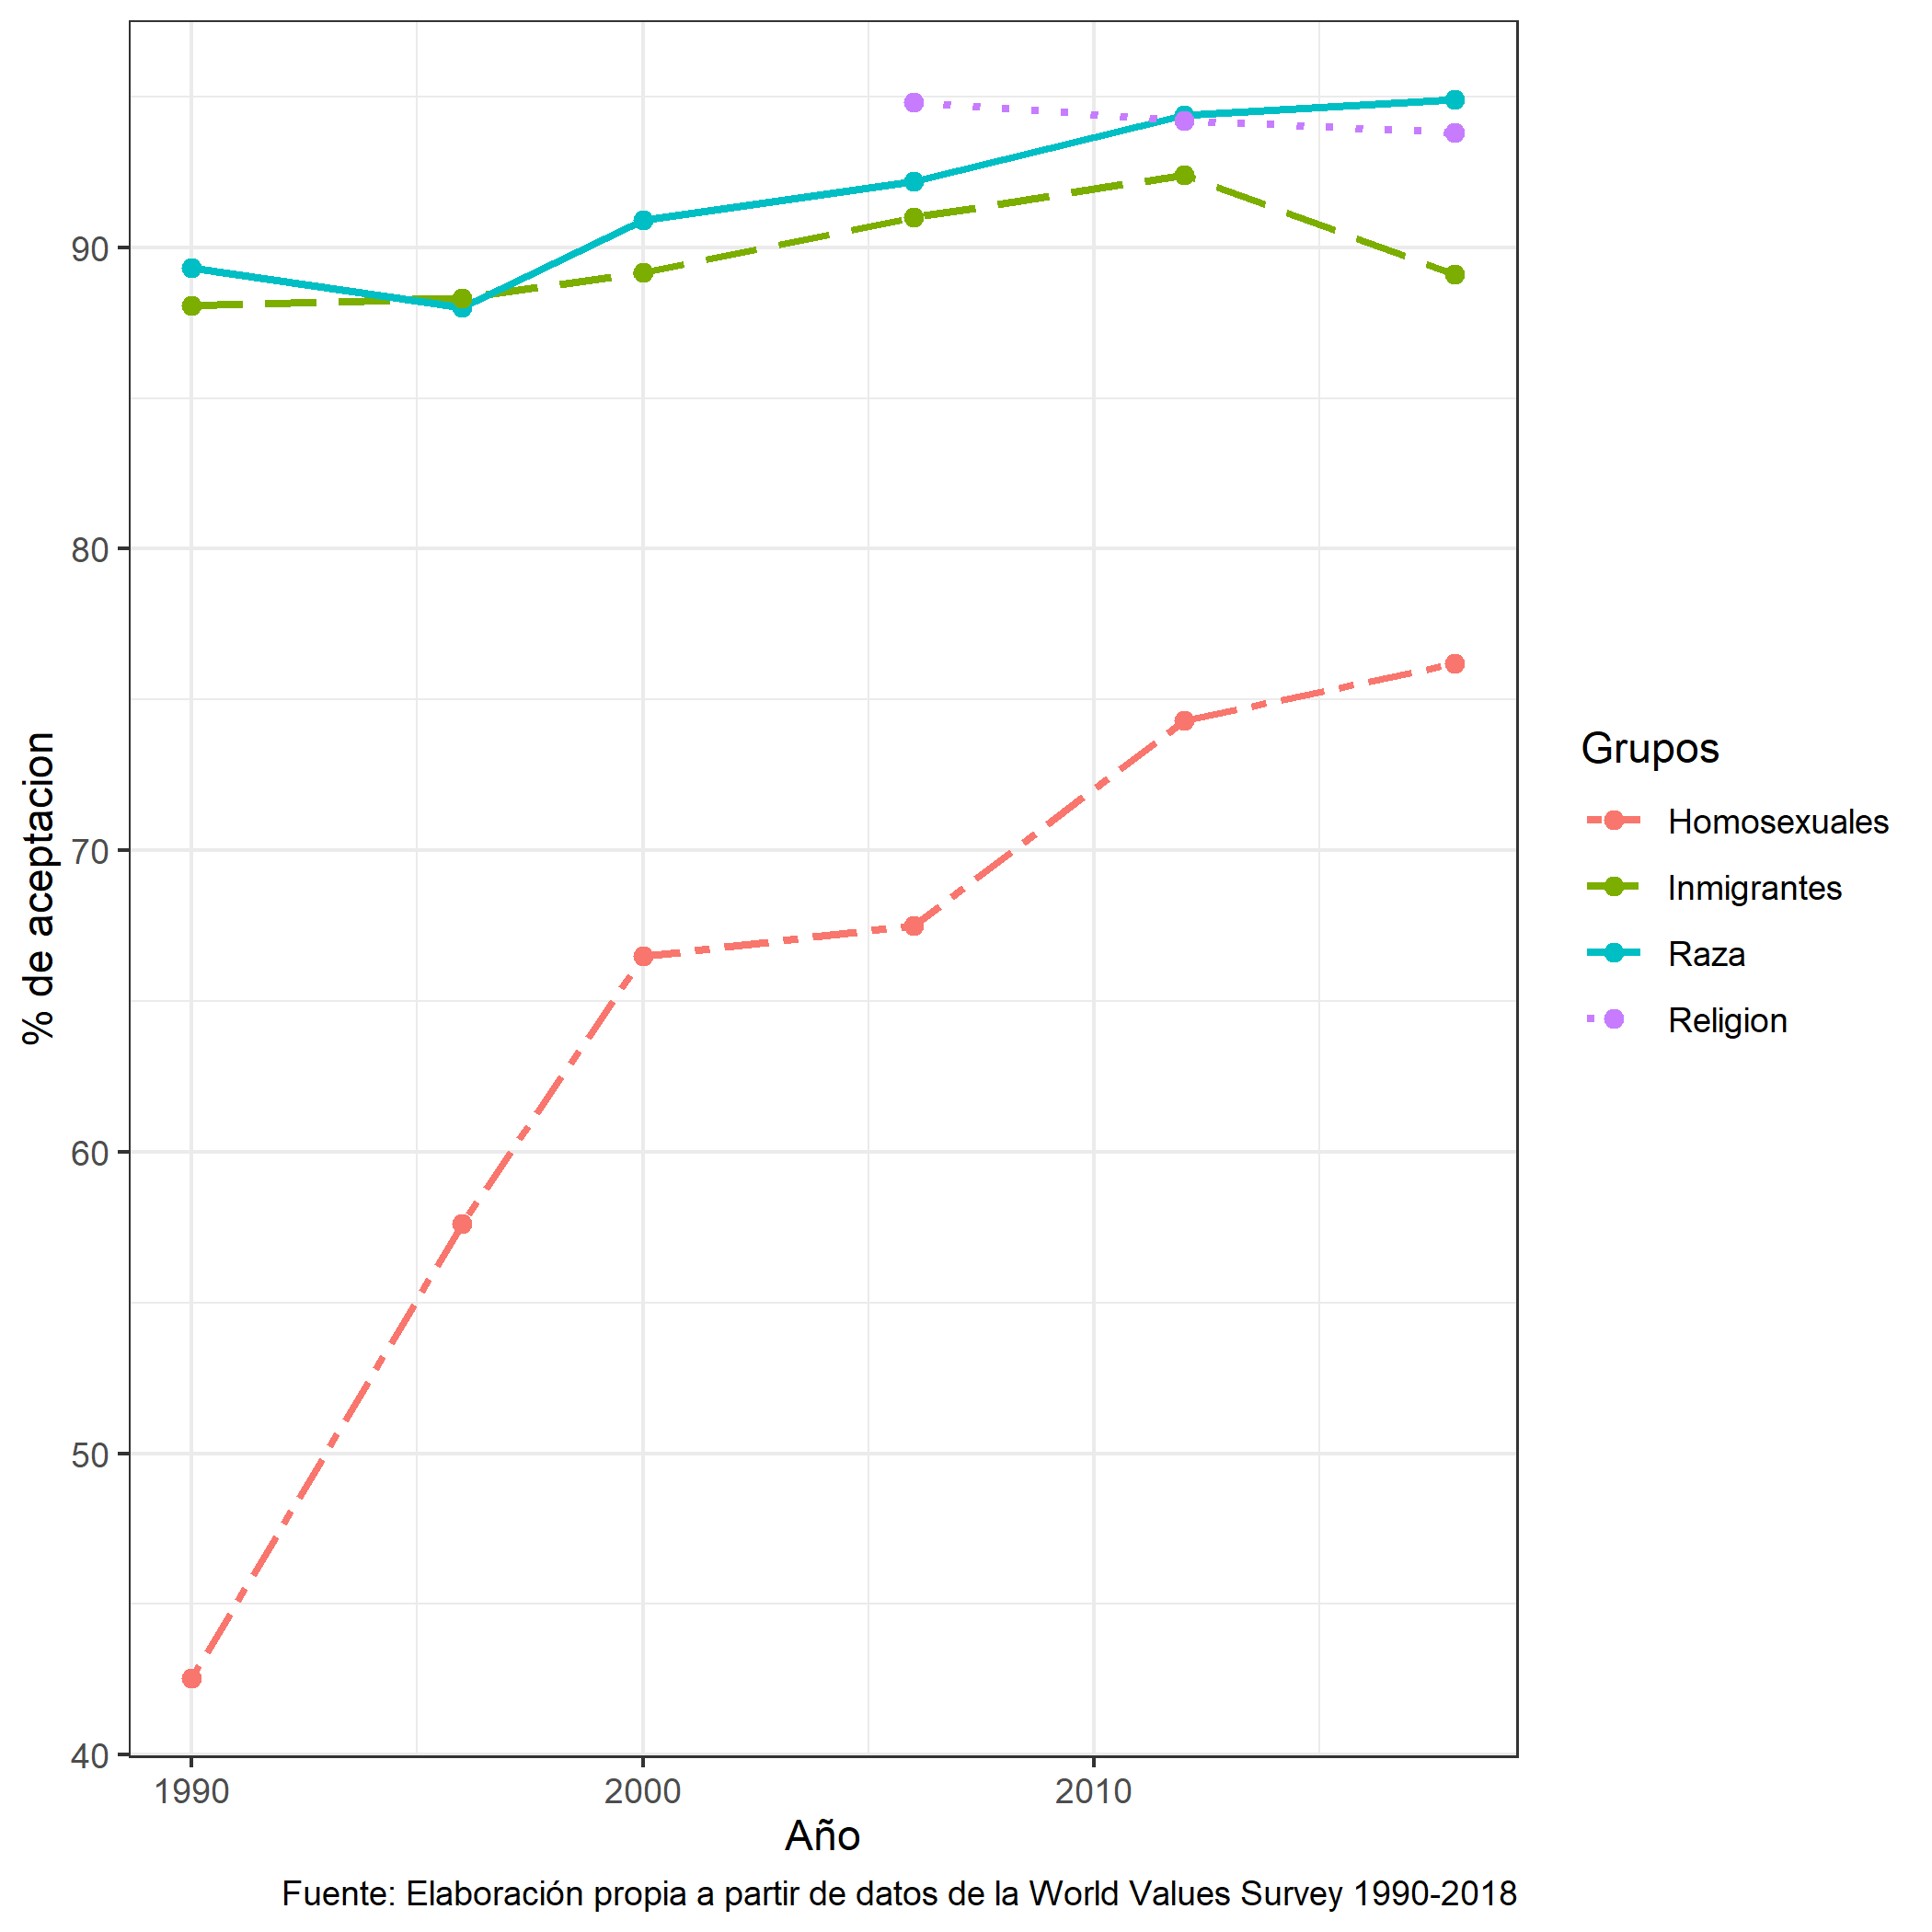
\includegraphics[width=1\linewidth]{images/aceptacion_wvs} 

}

\caption{Porcentaje de aceptación de distintos grupos sociales en población adulta de Chile}\label{fig:aceptacion-wvs}
\end{figure}

\textbf{Políticas educativas y los desafíos para la democracia actual}

Abordar el aprendizaje de actitudes hacia la aceptación social de jóvenes en edad escolar implica posicionar esta investigación bajo un incremento de la diversidad social que plantea importantes desafíos para los Estados-nación a nivel global en términos de políticas públicas, ya sea por sus implicancias gubernamentales, territoriales y socioeconómicas o por los nuevos requisitos que se originan en los distintos sistemas educativos a partir de demandas por inclusión y tolerancia de una población estudiantil diversa. En Chile se han suscrito distintos tratados internacionales que pretenden resguardar la diversidad (convenciones de DDHH, convenciones de Derechos del niño y el convenio 169 de la Organización Internacional del Trabajo) y que se han traducido en distintas políticas educativas que tienen por objetivo apoyar la inclusión de distintos sectores de la sociedad en el sistema educativo.

Dentro de este ámbito destacan la ley de inclusión escolar que regula, entre otras cosas, la admisión de los y las estudiantes en los establecimientos educativos \citep{bibliotecadelcongresonacional_ley_2015} y el Programa de Educación Intercultural Bilingüe (PEIB) que tiene sus orígenes en la década de 1990 y una consolidación entre 2010 y 2016 y que pretende generar las condiciones para que las comunidades educativas, que atienden a estudiantes indígenas y no indígenas, sean partícipes de procesos sociales inclusivos, que desarrollen nuevas competencias al considerar en sus procesos formativos otras formas de ver y entender el mundo y que reconozcan, valoren y se ajusten a estos orígenes culturales diversos \citep{ministeriodeeducacion_Programa_2017}.

Los aprendizajes que se le adjudican a la educación ciudadana en las escuelas pretenden dar respuesta a la necesidad de preparar a la nueva generación para la vida en democracia y sus requerimientos morales y cognitivos \citep{cox_objetivos_2015}. La nueva ley de Formación Ciudadana (ley n° 20.911) dispone que todos los establecimientos educacionales deben diseñar un Plan de Formación Ciudadana que brinde a los estudiantes la preparación necesaria para asumir una vida responsable en una sociedad libre y de orientación hacia el mejoramiento integral de la persona humana, como fundamento del sistema democrático, la justicia social y el progreso \citep{bibliotecadelcongresonacional_plan_2016}. Entre sus principales objetivos, esta nueva ley busca promover la comprensión y análisis del concepto de ciudadanía y los derechos y deberes asociados a ella, además de fomentar en los estudiantes la valoración de la diversidad social y cultural del país y fomentar en los estudiantes la tolerancia y el pluralismo \citep{bibliotecadelcongresonacional_plan_2016}.

Sin embargo, la tolerancia orientada hacia la existencia de una diversidad social marca una diferencia entre la aceptación, respeto y apreciación de la diferencia y la inclusión homogeneizante de los distintos grupos sociales dentro de las escuelas, ya que la definición de interculturalidad que se ha incluido en el sistema educativo es funcional al estatus quo al absorber a la diferencia y homogenizarlos \citep{riedemann_Desde_2020}. De esta forma, se invisibiliza y reproduce una discriminación basada en procesos de racialización, generización y diferenciación en términos de clase, acercándose más a la idea de multiculturalismo que a la de interculturalidad \citep{stefoni_Educacion_2016a}. Esta confusión en el horizonte de la educación intercultural produce una ineficacia de las políticas emprendidas y repercute en una incapacidad de generar una sociedad que acepte la diversidad y que establezca relaciones de cooperación entre sus diversidades \citep{donosoromo_INTERCULTURALIDAD_2006}. Lo anterior provoca que, en la práctica, antes que buscar una coexistencia de las diversidades, en el sistema educativo chileno se busca que los diferentes grupos sociales se integren a la sociedad nacional para que así obtengan los beneficios que ella reporta a todos sus ciudadanos \citep{donosoromo_INTERCULTURALIDAD_2006}. Esto provoca una contradicción en los establecimientos educacionales ya que se les pide valorar la diversidad social y cultural en las aulas mientras que, al mismo tiempo, se les exige responder a mecanismos de rendición de cuentas estandarizados que no dan cuenta de la diversidad \citep{riedemann_Desde_2020}.

De esta forma, si bien los procesos de socialización se han amplificado y complejizado junto con los procesos de modernización y globalización, el rol de la escuela y la familia siguen siendo los principales agentes de socialización. Para la sociología la comprensión de la educación como un agente de socialización de las generaciones más jóvenes resulta fundamental, mientras que el rol de la familia ha sido estudiado en menor medida dentro de esta disciplina, sino más bien desde la psicología social. Así, las investigaciones sobre tolerancia e inclusión en población juvenil frecuentemente se han enfocado en problemáticas relacionadas con los flujos migratorios y su inserción en el sistema educativo de cada país, centrándose en cómo las escuelas permiten el ingreso e inclusión de distintos estudiantes en el sistema educativo \citep{bellei_estudio_2013, ortiz_Actitudes_2016, stefoni_Educacion_2016a} o en cómo las escuelas son capaces de influir en la (in)tolerancia y prejuicio hacia inmigrantes, minorías étnicas o disidencias sexuales \citep{lee_Tolerated_2014, maurissen_Classroom_2020, trevino_Influence_2018}. En cuanto al rol de la familia, algunas investigaciones han dado cuenta del efecto de las actitudes de los padres en el conflicto interétnico de su descendencia \citep{medjedovic_intergroup_2021} y de la participación política parental en el compromiso político de las nuevas generaciones \citep{bacovsky_raising_2021}. Además, en sociedades desiguales como la chilena, los recursos socioeconómicos funcionan como un mecanismo de diferenciación a nivel general donde, por ejemplo, \citet{bellei_estudio_2013} ha dado cuenta del rol predominante de los recursos socioeconómicos de las familias como un agente diferenciador del logro académico.

Esta investigación pretende comprender cómo los diferentes modos de socialización se articulan entre sí y producen las disposiciones para excluir o aceptar a determinados grupos sociales. Así, la pregunta de investigación que guía este estudio es ¿en qué medida los distintos procesos de socialización son capaces de influir en las actitudes de las y los jóvenes estudiantes chilenos hacia la diversidad en su vecindario?

\hypertarget{objetivo-general}{%
\section{Objetivo general}\label{objetivo-general}}

Determinar en qué medida varían las actitudes de los/as estudiantes que se relacionan con la aceptación de distintos grupos sociales de sus vecindarios, así como analizar el rol que poseen la familia y la escuela como agentes de socialización política de actitudes en jóvenes estudiantes chilenos.

\hypertarget{objetivos-especuxedficos}{%
\section{Objetivos específicos}\label{objetivos-especuxedficos}}

\begin{enumerate}
\def\labelenumi{\arabic{enumi}.}
\item
  Determinar en qué medida los/as jóvenes estudiantes chilenos aceptan o rechazan que diferentes grupos sociales vivan en sus vecindarios.
\item
  Analizar el rol de la familia en la socialización política de actitudes hacia la diversidad social.
\item
  Analizar el rol de la escuela en la socialización política de actitudes hacia la diversidad social.
\end{enumerate}

\hypertarget{aceptar-la-diversidad-en-el-vecindario}{%
\chapter{Aceptar la diversidad en el vecindario}\label{aceptar-la-diversidad-en-el-vecindario}}

En Chile, las desigualdades interaccionales se han convertido en las desigualdades más percibidas y rechazadas por la población \citep{araujo_igualdad_2013}. Este tipo de desigualdades refieren a la manera en que las personas son tratadas por otros individuos o instituciones en las interacciones sociales ordinarias y concretas \citep{araujo_percepcion_2019}. Para \citet{araujo_percepcion_2019} se ha instalado una \emph{malignización de la otredad}, en que se constituye al otro como una amenaza y adversario, quebrando la noción de un espacio común y dando un marco de confrontación y disputa a las relaciones ordinarias entre los habitantes de la ciudad. De esta forma, \citet{castells_globalizacion_2005} indica que el principio identitario dominante en América Latina es la identidad nacional, construida en torno a un Estado-nación que impulsaba un proyecto de desarrollo y una especificidad frente al resto de los países. Así, en la medida en que el Estado-nación se inserta en la globalización y se despega de sus bases tradicionales, ``la separación entre Estado y nación lleva a una crisis de la identidad nacional como principio de cohesión social'' \citep[p.~40]{castells_globalizacion_2005}.

Como resultado, \citet{castells_globalizacion_2005} plantea que la identidad se convierte en un principio débil que no basta para construir el sentido de la vida colectiva y son suplantadas por el individualismo legitimado por el mercado, que se convierte en fuente de racionalidad y de proyecto, a la vez que se crean identidades comunitarias más fuertes, lo que conlleva el resurgimiento de la religión o identidades étnicas. Ante esta problemática, la Teoría de la Identidad Social ofrece un marco conceptual que permite explicar los procesos grupales y las relaciones intergrupales en términos de la interacción de los procesos sociales cognitivos, interactivos y societarios, en el que se ubica la autoconcepción identitaria en el centro de esta dinámica \citep{hogg_social_2016}. Esta interacción intergrupal se concibe como un recurso funcional que emerge en el seno de condicionantes contextuales e individuales concretos con el objeto de proporcionar a cada individuo las estrategias necesarias para afirmar su identidad \citep{scandroglio_teoria_2008}. Así, esta construcción de una identidad social define y evalúa el autoconcepto de uno mismo y cómo será tratado y pensado por los demás y, por lo tanto, cuando las personas hacen comparaciones entre su propio grupo y un grupo externo, se preocupan por asegurarse de que su propio grupo sea positivamente distintivo, claramente diferenciado y evaluado más favorablemente que los grupos externos \citep{hogg_social_2016}.

De esta forma, la exclusión o rechazo de diferentes grupos sociales de un vecindario se comprende como una forma de cierre social en que se establecen barreras entre sectores o clases a partir de la construcción de identidades, comunidades y la monopolización de oportunidades con el fin de excluir a otras personas de ese círculo o clase \citep{parkin_Marxismo_1984}. En esta misma línea, \citet{tilly_desigualdad_2000} plantea que en cada sociedad existen desigualdades persistentes, ya que las desigualdades por ``raza, género, etnia, clase, edad, ciudadanía, nivel educacional y otros principios de diferenciación aparentemente contradictorios, se forman mediante procesos sociales similares y son, en una medida importante, organizacionalmente intercambiables'' \citep[p.~23]{tilly_desigualdad_2000}. Por un lado, estas desigualdades, más allá de las frecuentes formas de violencia explícitamente racista, tienden a materializarse en no tener acceso o tener un acceso menor al país, ciudad, barrio, vivienda, bares, política y/o medios de comunicación \citep{vandijk_Racismo_2013}. \citet{vandijk_Racismo_2013} señala que se trata de una práctica social diferenciada, generalmente denominada discriminación, que se basa en prejuicios e ideologías racistas sobre la superioridad de una mayoría y la inferioridad de una minoría. Por otro lado, \citet{diez-nicolas_Exclusion_2019} plantean que se trata de formas de exclusión social que frecuentemente se relacionan con conceptos como estigma, discriminación y prejuicio. No obstante, reducir o intensificar ciertas actitudes tendrá poco efecto sobre estas desigualdades persistentes, por lo que el foco debe estar puesto en los mecanismos sociales que producen esta desigualdad \citep{tilly_desigualdad_2000}.

Medir la (in)tolerancia es un debate sostenido dentro de distintas disciplinas, que generalmente confluyen en dos enfoques centrales. Por un lado, se ha propuesto medir la tolerancia hacia grupos subalternos tales como migrantes, minorías étnicas y mujeres a partir de un enfoque de derechos \citep{miranda_Political_2018, trevino_Influence_2018}, de prejuicios \citep{meeusen_ParentChild_2015, weber_educational_2020} y como una amenaza material y/o simbólica \citep{raijman_Perceived_2004}. Por otro lado, \citet{diez-nicolas_Exclusion_2019} plantean que se trata de formas de exclusión social que frecuentemente se relacionan con conceptos como estigma, discriminación y prejuicio. Asimismo, \citet{tendam_Measuring_2011} proponen que, para jóvenes, las actitudes de ciudadanía se manifiestan en las tareas sociales cotidianas. En la presente investigación se propone medir la tolerancia a partir de la aceptación o rechazo de que distintos grupos sociales vivan en el mismo vecindario que los estudiantes encuestados. Aceptar la diversidad en el vecindario refiere, por lo tanto, a formas de no exclusión de distintos grupos subalternos tradicionalmente marginados de la esfera social. En concreto, esta perspectiva teórica permite abordar si los estudiantes aceptan o rechazan que vivan en su vecindario personas de origen indígena, de distinto país, distinta región, distinta orientación sexual, distinta clase social, distinto color de piel y distinta religión.

\hypertarget{procesos-de-socializaciuxf3n-poluxedtica-de-actitudes}{%
\section{Procesos de socialización política de actitudes}\label{procesos-de-socializaciuxf3n-poluxedtica-de-actitudes}}

A través de procesos de socialización diferenciados y continuos en el tiempo se producen distintos condicionamientos asociados a una clase particular de condiciones de existencia \citep{bourdieu_sentido_2007}. A partir de esto, si bien los planteamientos de \citet{bourdieu_sentido_2007} podrían explicar la disposición de los individuos a generar y reproducir prácticas de exclusión social hacia distintos grupos sociales, no permiten comprender el modo en que se generan estas disposiciones. Es así como \citet{archer_teoria_2009} plantea la problemática que ha tenido la sociología de la educación al centrarse solo en las prácticas y procesos que ocurren dentro de la escuela y no reconocer que ``tanto los profesores como los alumnos están inmersos en relaciones socioculturales más amplias que traen consigo a la sala de clase'' \citep[p.~39]{archer_teoria_2009}. Esto implica que existe una interacción entre el contexto y las actividades sociales, pero que estas no covarían en el tiempo, sino que están desfasadas la una de la otra. Para \citet{lahire_teoria_2012} resulta relevante comprender el mundo social a escala del individuo al mismo tiempo que se comprenden las condiciones sociales (y discursivas) de producción del individuo moral e ideológico, porque son elementos socialmente producidos. En este caso, el objetivo de esta investigación es comprender cómo los diferentes modos de socialización se articulan entre sí y producen las disposiciones para excluir o aceptar a determinados grupos sociales, ya que ``los individuos socializados pueden haber interiorizado de manera duradera un cierto número de hábitos y, sin embargo, no tener ningún deseo particular de aplicarlos'' \citep[p.~87]{lahire_teoria_2012}.

Para la sociología en general y la sociología de la educación en particular, la articulación de los procesos de socialización se concebirían como una sociología de los modos de socialización (escolares y extraescolares), articulándose con una sociología del conocimiento, para así poder comprender a grandes rasgos una disposición a partir de la reconstrucción de su génesis \citep{lahire_teoria_2012}. Esto es, abordar de manera articulada el rol de la familia y la escuela en la socialización política de actitudes hacia la diversidad social y el contexto en que estas se producen.

Al articular los diferentes modos de socialización, \citet{aedohenriquez_habitus_2015} señala que es relevante tener en consideración la idea de Estrategia de Bourdieu, ya que esta implica ponerse a sí mismo en relación con otros, en situaciones propias del campo, en que las expectativas socializadas sobre su posición con respecto a otros entran en interrogación. La idea de Estrategia de Bourdieu refiere a que ``en el mundo social actuamos conforme a ciertas inclinaciones que hemos incorporado a lo largo de nuestra experiencia social, en el marco de los procesos de socialización, inclinaciones o disposiciones que actúan como facilitadores de nuestras prácticas o de nuestros actos'' \citep[p.~280]{aguilar_habitus_2017}.

Así, los grupos familiares estratégicamente seleccionan escuelas y vecindarios en los que integrar a sus hijos de acuerdo con sus disposiciones, esto es, que son capaces de elegir el espacio social en que socializarán a sus hijos. De la misma forma, la disposición hacia la exclusión -y hacia el cierre social que conlleva- marcaría dos momentos temporales. Por un lado, refiere a una expresión de los procesos de socialización familiares previos y, por otro lado, expresan las condiciones familiares objetivas que condicionan el proceso de socialización actual.

\hypertarget{socializaciuxf3n-poluxedtica-familiar-de-actitudes-hacia-la-diversidad-social.}{%
\subsection{Socialización política familiar de actitudes hacia la diversidad social.}\label{socializaciuxf3n-poluxedtica-familiar-de-actitudes-hacia-la-diversidad-social.}}

El proceso de socialización política familiar se concibe como prácticas de crianza o estrategias de socialización concretas que buscan modelar las conductas de sus hijos e hijas según las propias valoraciones y personalidades que se estimen como positivas para la integración y el desenvolvimiento social en el futuro \citep{ramirez_padres_2005}. De esta forma, las familias reproducen y socializan valores a través de un proceso de transmisión de actitudes que permite asegurar la perpetuación del grupo social y la conservación del estatus y el privilegio \citep{bourdieu_reproduccion_1998, bernstein_theoretical_2005}.

Dentro de las estrategias del proceso de socialización política familiar se han reconocido dos elementos. En primer lugar, \citet{lipset_hombre_1997} plantea la importancia de las condiciones socioeconómicas objetivas de la familia en el proceso de adquisición de valores y prácticas democráticas. En segundo lugar, para \citet{bandura_sociallearning_1969} la teoría del aprendizaje social implica que las actitudes y comportamientos de los padres inciden sobre los intereses y modos de comportamiento de sus hijos, planteando así la necesidad de estudiar la transmisión intergeneracional de actitudes como proceso de socialización.

En este sentido, diferentes investigaciones han dado cuenta del rol predominante que poseen los recursos socioeconómicos como condicionante de las expectativas de participación política de los estudiantes \citep{castillo_Social_2014} y, específicamente, sobre las actitudes de los estudiantes hacia uno o más grupos subalternos según el grado de tolerancia \citep{farkac_Tolerance_2020}, de prejuicios \citep{weber_educational_2020} o hacia la igualdad de derechos \citep{isac_Native_2012, miranda_Political_2018}. Por un lado, \citet{miranda_Political_2018} demuestran la importancia que posee el nivel educativo de los padres, el estatus ocupacional y la cantidad de libros en el hogar en la generación de actitudes positivas de los estudiantes hacia la igualdad de género y el estatus ocupacional de los padres y la cantidad de libros en el hogar sobre las actitudes hacia la igualdad de derechos para inmigrantes y minorías étnicas. Asimismo, \citet{ortiz_Actitudes_2016} demuestra la importancia que poseen estos tres indicadores sobre las actitudes hacia la tolerancia social en general, mientras que \citet{castillo_Social_2014} demuestran que padres con educación universitaria y la cantidad de libros en el hogar juegan un rol preponderante en las expectativas de participación política de los estudiantes. Por otro lado, \citet{sincer_relationship_2020} demuestran que una mayor proporción de estudiantes de bajo nivel socioeconómico en las escuelas influyen negativamente en las competencias para lidiar con las diferencias sociales\footnote{\citet{sincer_relationship_2020} señalan que \emph{dealing with differences} refiere al conocimiento, actitudes y habilidades para interactuar con las diferencias sociales.}. Por último, sobre la transmisión intergeneracional de actitudes, se ha dado cuenta de la preponderancia de las actitudes de los padres en la disposición hacia el conflicto interétnico de sus hijos \citep{medjedovic_intergroup_2021}, de cómo el historial de participación política parental influye en el compromiso político de las nuevas generaciones \citep{bacovsky_raising_2021} y que las familias de clase alta tienden a privilegiar valores más simbólico-relacionales, como los buenos modales y el respeto por los demás, mientras que las clases bajas privilegiarían transmitir valores de ascenso social, como el trabajo duro y el ahorro \citep{santanderramirez_preferencias_2020}. De esta forma, el proceso de socialización política familiar se refleja en las siguientes hipótesis:

\begin{itemize}
\item
  H1: Estudiantes que provienen de familias con mayores recursos socioeconómicos poseen un mayor grado de aceptación de la diversidad en sus vecindarios, manteniendo el resto de las variables constantes.
\item
  H2: Estudiantes que provengan de familias en que sus padres acepten en mayor medida que distintos grupos sociales vivan en sus vecindarios, poseerán un mayor grado de aceptación de la diversidad en sus vecindarios, manteniendo el resto de las variables constantes.
\end{itemize}

\hypertarget{socializaciuxf3n-poluxedtica-de-actitudes-hacia-la-diversidad-social-en-la-escuela.}{%
\subsection{Socialización política de actitudes hacia la diversidad social en la escuela.}\label{socializaciuxf3n-poluxedtica-de-actitudes-hacia-la-diversidad-social-en-la-escuela.}}

Dentro de la investigación sobre socialización política de actitudes en la escuela se tiende a adjudicar al sistema educacional el objetivo de ``suscitar y desarrollar al niño cierto número de estados físicos, intelectuales y morales que requieren en él tanto la sociedad política en su conjunto como el medio ambiente específico al que está especialmente destinado'' \citep[p.~60]{durkheim_educacion_1999}, y que la función socializadora de la escuela se resume en que ``consiste en el desarrollo dentro de cada individuo de aquellas habilidades y actitudes que constituyen los requisitos esenciales para su futuro desenvolvimiento en la vida'' \citep[p.~65]{parsons_clase_1976}. En esta línea, investigaciones recientes continúan enmarcándose en este rol de la escuela como agente formador de ciudadanos \citep{cox_Aprendizaje_2015, groof_Influence_2008, trevino_Influence_2017}, resaltando las capacidades que tienen las escuelas para contribuir en el desarrollo cívico y las actitudes democráticas de los jóvenes estudiantes.

La escuela se comprende como el espacio primordial de socialización y de encuentro entre personas de distintas realidades, funcionando como una micro sociedad \citep{groof_Influence_2008}. Las características estructurales de las escuelas son una dimensión clave para explicar los diferentes resultados que poseen los estudiantes \citep{trevino_Influence_2018}. En cierta medida esto se explica por la forma en que los estudiantes de diferentes estratos socioeconómicos se distribuyen a través de las escuelas según su tipo de administración \citep{bellei_estudio_2013} y por los conocimientos, habilidades y valores sociales que estas instituciones le logran otorgar a sus estudiantes \citep{groof_Influence_2008}. Específicamente, tanto las escuelas como las salas de clases pueden diferir entre sí en cuanto a sus valores y normas comunes, en cómo los estudiantes interactúan entre sí y cómo los profesores se acercan y tratan a los estudiantes \citep{bayramozdemir_How_2020}.

En primer lugar, el conocimiento cívico y las oportunidades que brinden las escuelas para su aprendizaje es un elemento esencial para la socialización de valores y normas comunes. El conocimiento cívico refiere a la información cívica y ciudadana aprendida que los estudiantes utilizan cuando se involucran en tareas más complejas que les ayudan a entender de mejor forma el mundo político \citep{carstens_Overview_2018}, mientras que \citet{sampermans_Back_2020} señalan que el conocimiento cívico depende directamente de las oportunidades de aprendizaje cívico que logren promover las escuelas. Diversos autores han demostrado que el conocimiento cívico influye de manera positiva sobre las actitudes de estudiantes hacia la tolerancia de personas inmigrantes \citep{isac_Native_2012, groof_Influence_2008, torney-purta_How_2008}.

En segundo lugar, una de las características estructurales fundamentales de las escuelas es la disposición de espacios de discusión. En las aulas donde los estudiantes están expuestos al mundo real de los problemas políticos, por medio del discurso y el debate tienen la oportunidad de luchar por cuestiones políticas y sociales, aprendiendo el elemento vital de la democracia participativa \citep{campbell_Voice_2008}. Por lo tanto, es evidente que esto solo se puede lograr cuando se promueve y se resguarda que exista comunicación y diálogo entre los alumnos de diferentes nacionalidades, etnias, lenguas, colores de piel, estratos socioeconómicos e intereses \citep{riedemann_Desde_2020}. Se ha demostrado que este indicador influye sobre las actitudes de los estudiantes hacia la tolerancia de inmigrantes \citep{eckstein_school_2021, maurissen_Classroom_2020, groof_Influence_2008, isac_Native_2012}, sobre las actitudes de los estudiantes hacia la igualdad de derechos para inmigrantes, minorías étnicas y mujeres \citep{trevino_Influence_2018, trevino_Influence_2017}, sobre las actitudes cívicas de los estudiantes en general \citep[ \citet{trolian_shaping_2022}]{barber_Profiles_2020} y sobre la formación de conocimiento cívico en los estudiantes \citep{sampermans_Back_2020, barber_Immigrant_2015}. De esta forma, el rol de la escuela en la socialización política de actitudes se resume en las siguientes hipótesis:

\begin{itemize}
\item
  H3: Estudiantes que poseen un mayor conocimiento cívico presentan un mayor grado de aceptación de la diversidad en sus vecindarios, manteniendo el resto de las variables constantes.
\item
  H4: Estudiantes que perciben una mayor apertura a la discusión en sus aulas presentan un mayor grado de aceptación de la diversidad en sus vecindarios, manteniendo el resto de las variables constantes.
\end{itemize}

Finalmente, debido al rol del sistema educacional al alero de las nuevas políticas públicas de inclusión y Educación ciudadana, de manera exploratoria se plantea que las escuelas son capaces de mitigar las desigualdades sociales de origen y/o potenciar las actitudes positivas en la formación de las actitudes de los estudiantes hacia la aceptación de la diversidad en sus vecindarios. Esto implica que las escuelas cumplen un rol moderador en la generación de las actitudes de los estudiantes y, por lo tanto, se plantea la siguiente hipótesis:

\begin{itemize}
\tightlist
\item
  H5: El proceso de socialización en las escuelas cumple un rol moderador sobre la influencia de la socialización de la familia en las actitudes de los estudiantes hacia la aceptación de la diversidad en sus vecindarios.
\end{itemize}

\hypertarget{implicancias-del-vecindario-en-la-socializaciuxf3n-poluxedtica-de-actitudes-hacia-la-diversidad-social.}{%
\subsection{Implicancias del vecindario en la socialización política de actitudes hacia la diversidad social.}\label{implicancias-del-vecindario-en-la-socializaciuxf3n-poluxedtica-de-actitudes-hacia-la-diversidad-social.}}

El incremento de la diversidad social en los vecindarios tiene distintos efectos sobre la convivencia social y la tolerancia de lo que se percibe como diferente. Por un lado, en vecindarios heterogéneos, con una mayor diversidad de contactos sociales y una mayor interacción entre individuos de diversos orígenes, se deberían generar las condiciones para tener un mayor grado de prosocialidad \citep{diprete_segregation_2011}, sin embargo, también se ha argumentado que una mayor interacción entre grupos distintos podría reforzar los prejuicios \citep{putnam_pluribus_2007}. Por otro lado, la marcada segregación urbana del contexto chileno que sienta las bases para la consolidación de vecindarios homogéneos es bastante desfavorable para el contacto intergrupal positivo y la reducción de prejuicios \citep{garreton_city_2017}. En esta misma línea, \citet{garreton_social_2021} muestran que el capital social, es decir, una mayor cantidad de vínculos y contactos positivos, está negativamente correlacionado con la diversidad socioeconómica, pero positivamente correlacionado con una mayor diversidad de inmigrantes, lo que sugiere la importancia de diferenciar ambos contextos en el desarrollo del capital social.

En cada vecindario, los distintos patrones de segregación están asociados con grandes diferencias en el acceso al mercado laboral y a otros recursos culturales y sociales \citep{fernandez_breaking_2016}. Así, según \citet{baldassarri_diversity_2020}, la competencia entre \emph{minorías} es mayor en los lugares donde estas son más numerosas. Esto se debe a que las minorías étnicas y raciales a menudo no pueden competir por trabajos de alta calidad, incluso estando calificadas para ellos, y en su lugar se ven obligadas a competir por trabajos de menor calidad o informales, lo que trae como consecuencia que las personas de clases sociales bajas puedan sentir a las minorías como amenazas con más frecuencia que la gente de clases sociales más altas \citep{baldassarri_diversity_2020}. Este sentimiento de amenaza producido por la competencia por recursos y trabajos tiende a disminuir la confianza entre grupos distintos, dificultando así el desarrollo de vínculos sociales \citep{cote_untangling_2009}.

De esta forma, las características específicas de cada vecindario podrían afectar de diferentes maneras las actitudes de los y las estudiantes, dependiendo de sus condiciones materiales, de la disponibilidad de recursos y de la calidad y cantidad de los contactos e interacciones con personas de diferentes grupos. Por ejemplo, se ha estudiado que una mayor segregación residencial se asocia con actitudes negativas hacia inmigrantes y en personas nativas de territorios donde ha habido un gran cambio en la diversidad en los últimos años \citep{kawalerowicz_too_2021}, el entorno físico del vecindario, como la accesibilidad a diferentes tipos de espacios públicos urbanos contribuye a una actitud más positiva hacia la inclusión de inmigrantes al fomentar una interacción vecinal más fuerte \citep{wang_neighborhood_2022} o que en territorios con alta confianza en extranjeros esta no se relaciona con la proporción de inmigrantes en la población del vecindario \citep{schonwalder_attitudes_2016}. Sin embargo, algunos de estos elementos escapan de los alcances de esta investigación y de la disponibilidad de datos, por lo que se plantean tres hipótesis sobre características de los vecindarios que podrían afectar si los y las estudiantes aceptan o rechazan que distintos grupos sociales vivan en sus vecindarios:

\begin{itemize}
\item
  H6: Estudiantes que viven en vecindarios con una mayor proporción de personas que se identifican con alguna etnia presentan un menor grado de aceptación de la diversidad en sus vecindarios, manteniendo el resto de las variables constantes.
\item
  H7: Estudiantes que viven en vecindarios con una mayor proporción de población inmigrante presentan un menor grado de aceptación de la diversidad en sus vecindarios, manteniendo el resto de las variables constantes.
\item
  H8: Estudiantes que viven en vecindarios con un mayor promedio de escolaridad presentan un mayor grado de aceptación de la diversidad en sus vecindarios, manteniendo el resto de las variables constantes.
\end{itemize}

\hypertarget{muxe9todo}{%
\chapter{Método}\label{muxe9todo}}

\hypertarget{datos}{%
\section{Datos}\label{datos}}

La base de datos a utilizar corresponde al Primer Estudio de Educación Ciudadana en Chile, realizado por la Agencia de Calidad de la Educación del Ministerio de Educación. En este estudio se evaluaron 8.589 estudiantes de octavo básico provenientes de 242 escuelas. La fecha de aplicación fue el 9 de noviembre de 2017. También se utilizarán las preguntas del cuestionario de Formación Ciudadana con las respuestas de 6.770 apoderados. Al juntar ambas bases de datos, el N total de respuestas completas es de 6.511 estudiantes y apoderados. El N final utilizado en los análisis es de 4.801 casos.

Sumado a lo anterior, para las variables del territorio se utilizará la base de datos del CENSO 2017, obtenida a partir del paquete estadístico de R \emph{censo2017} \citep{vargas_censo2017_2022}. Esta base de datos contiene información respecto de datos territoriales asociados al año 2017 y se encuentra disponible para su libre uso.

\hypertarget{variables}{%
\section{Variables}\label{variables}}

Con el fin de medir las actitudes de los y las estudiantes hacia la diversidad en sus vecindarios se utiliza la batería de preguntas del módulo ``Tolerancia y Distancia Social'' del cuestionario de estudiantes. Estas variables están medidas a partir de las preguntas que se presentan en la Figura \ref{fig:dep-est}.

\begin{figure}[!ht]

{\centering 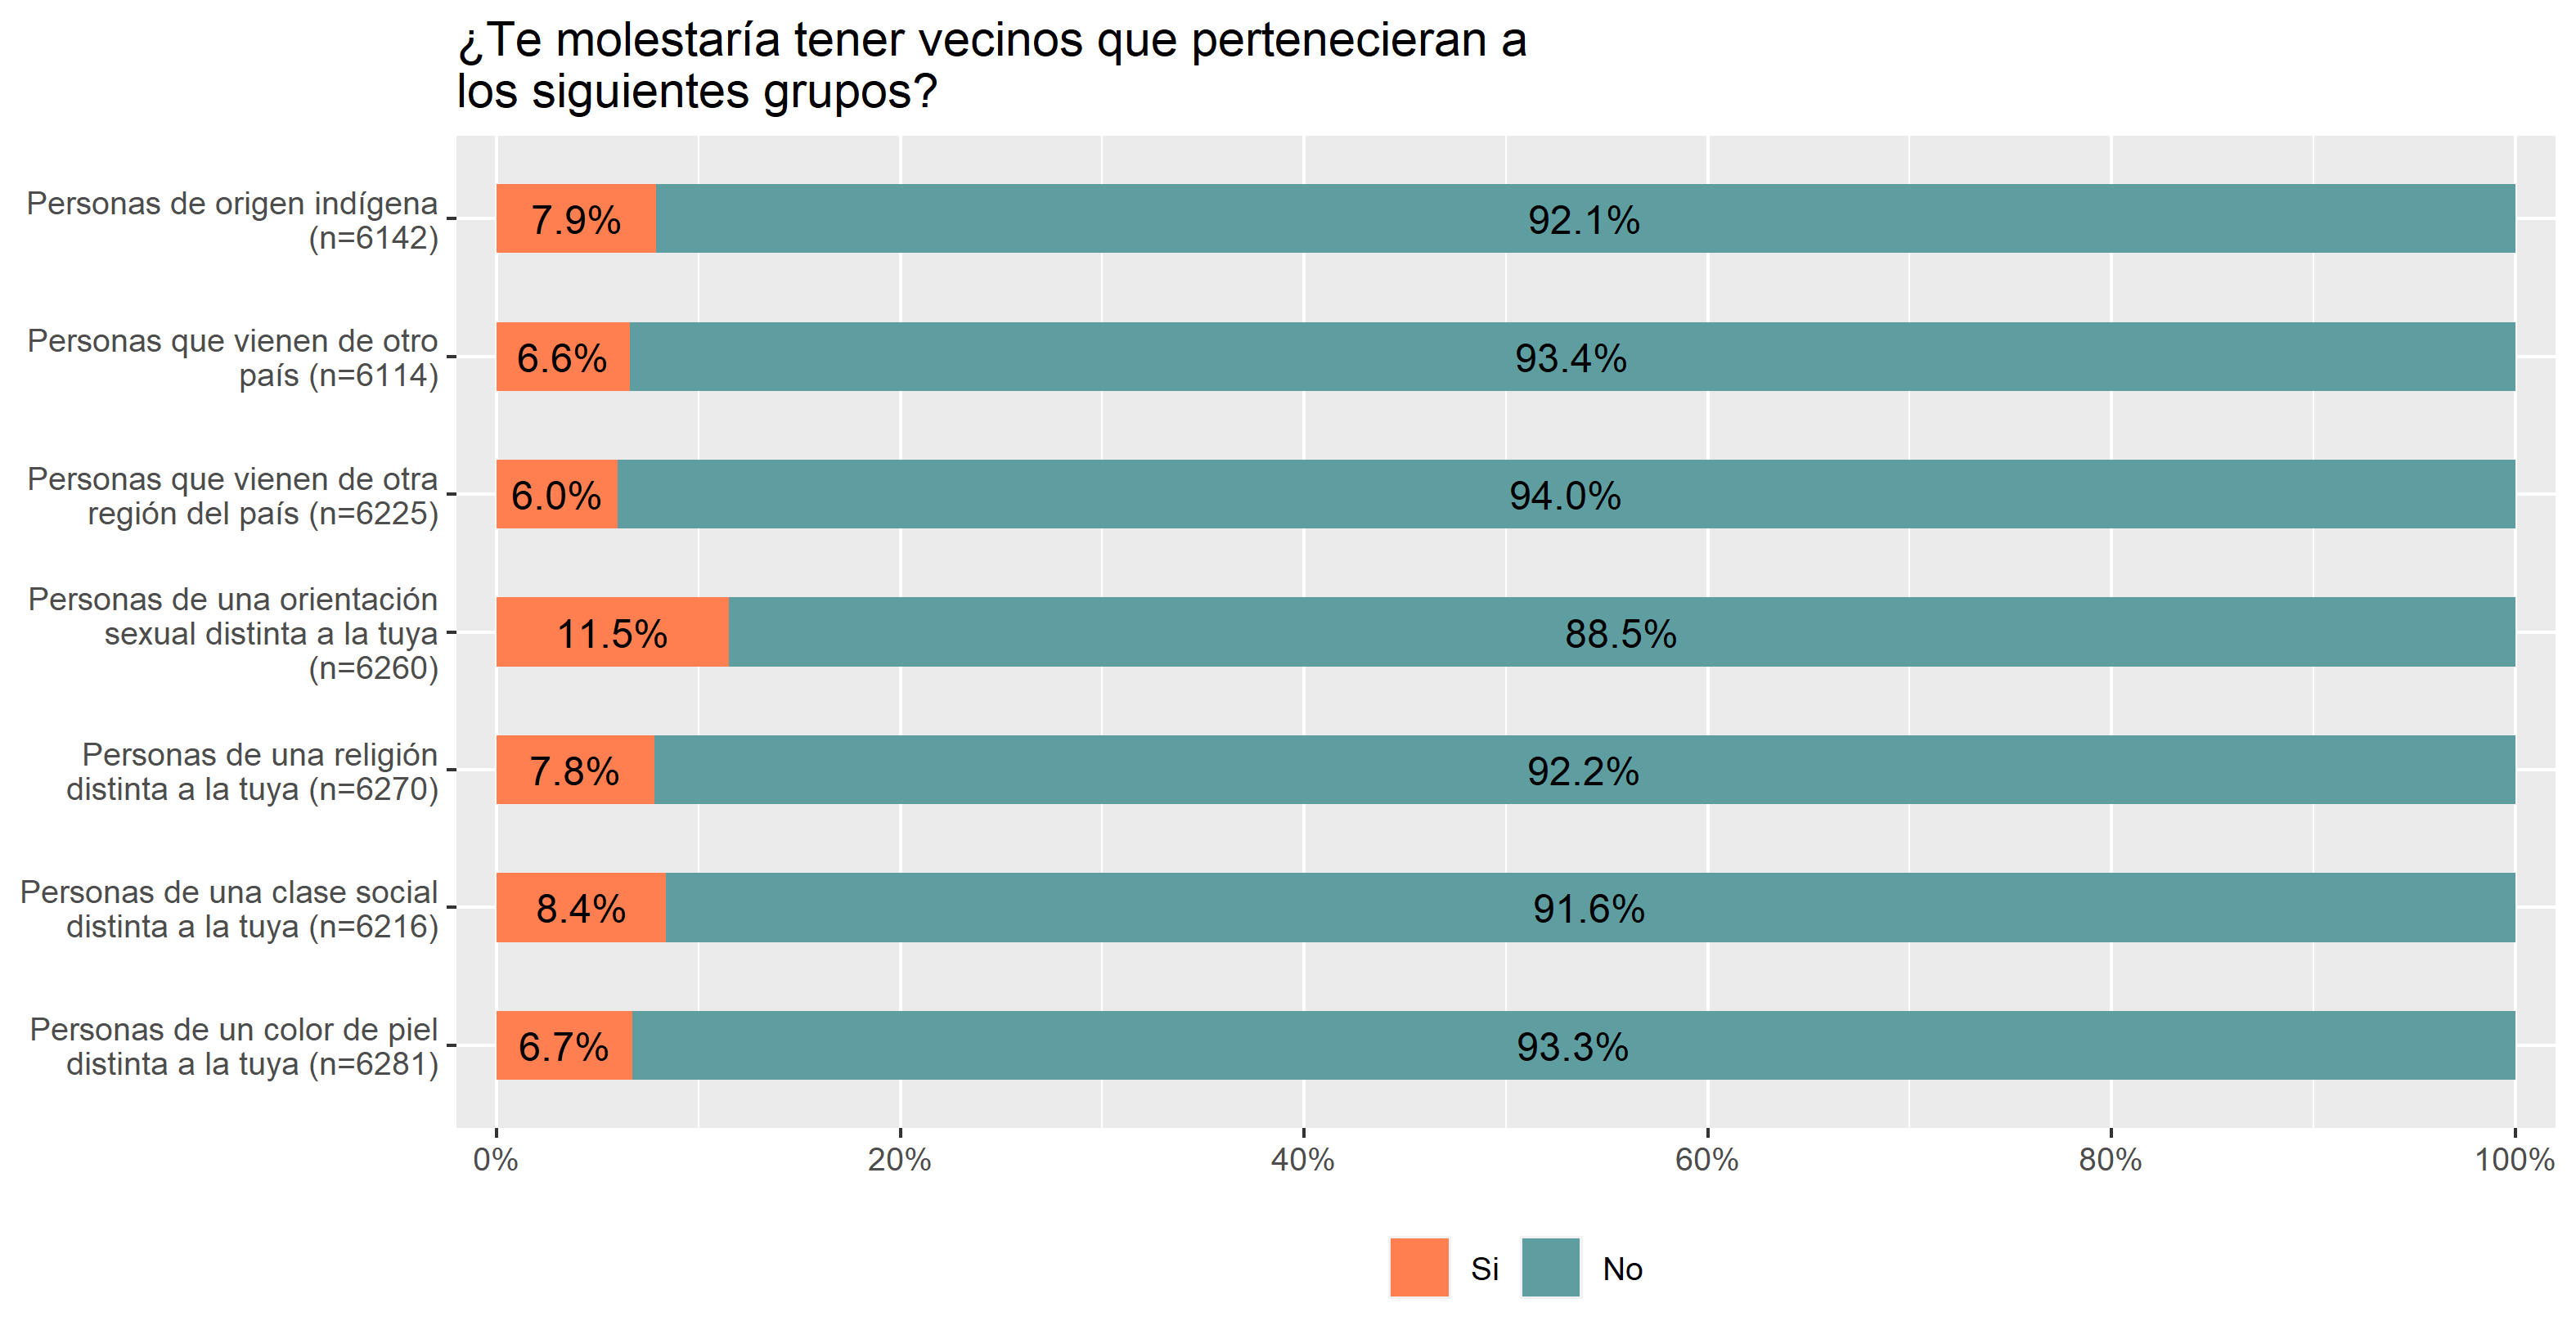
\includegraphics[width=0.8\linewidth,]{IPO/output/graphs/div_est} 

}

\caption{Aceptacion de la diversidad (estudiantes)}\label{fig:dep-est}
\end{figure}

Para operacionalizar esta batería de preguntas, en primer lugar, se recodificarán los ítems de modo que 0 indique que no le gustaría que cada uno de los grupos viva en su vecindario y 1 indique que sí le gustaría. Luego, se construirá un índice sumativo a partir de la suma de los ítems para representar el grado de aceptación de todos los grupos. La distribución de este índice se puede observar en el Gráfico \ref{fig:ind-est}. El valor de Alpha de Cronbach de este índice es de 0.887

\begin{figure}[!ht]

{\centering 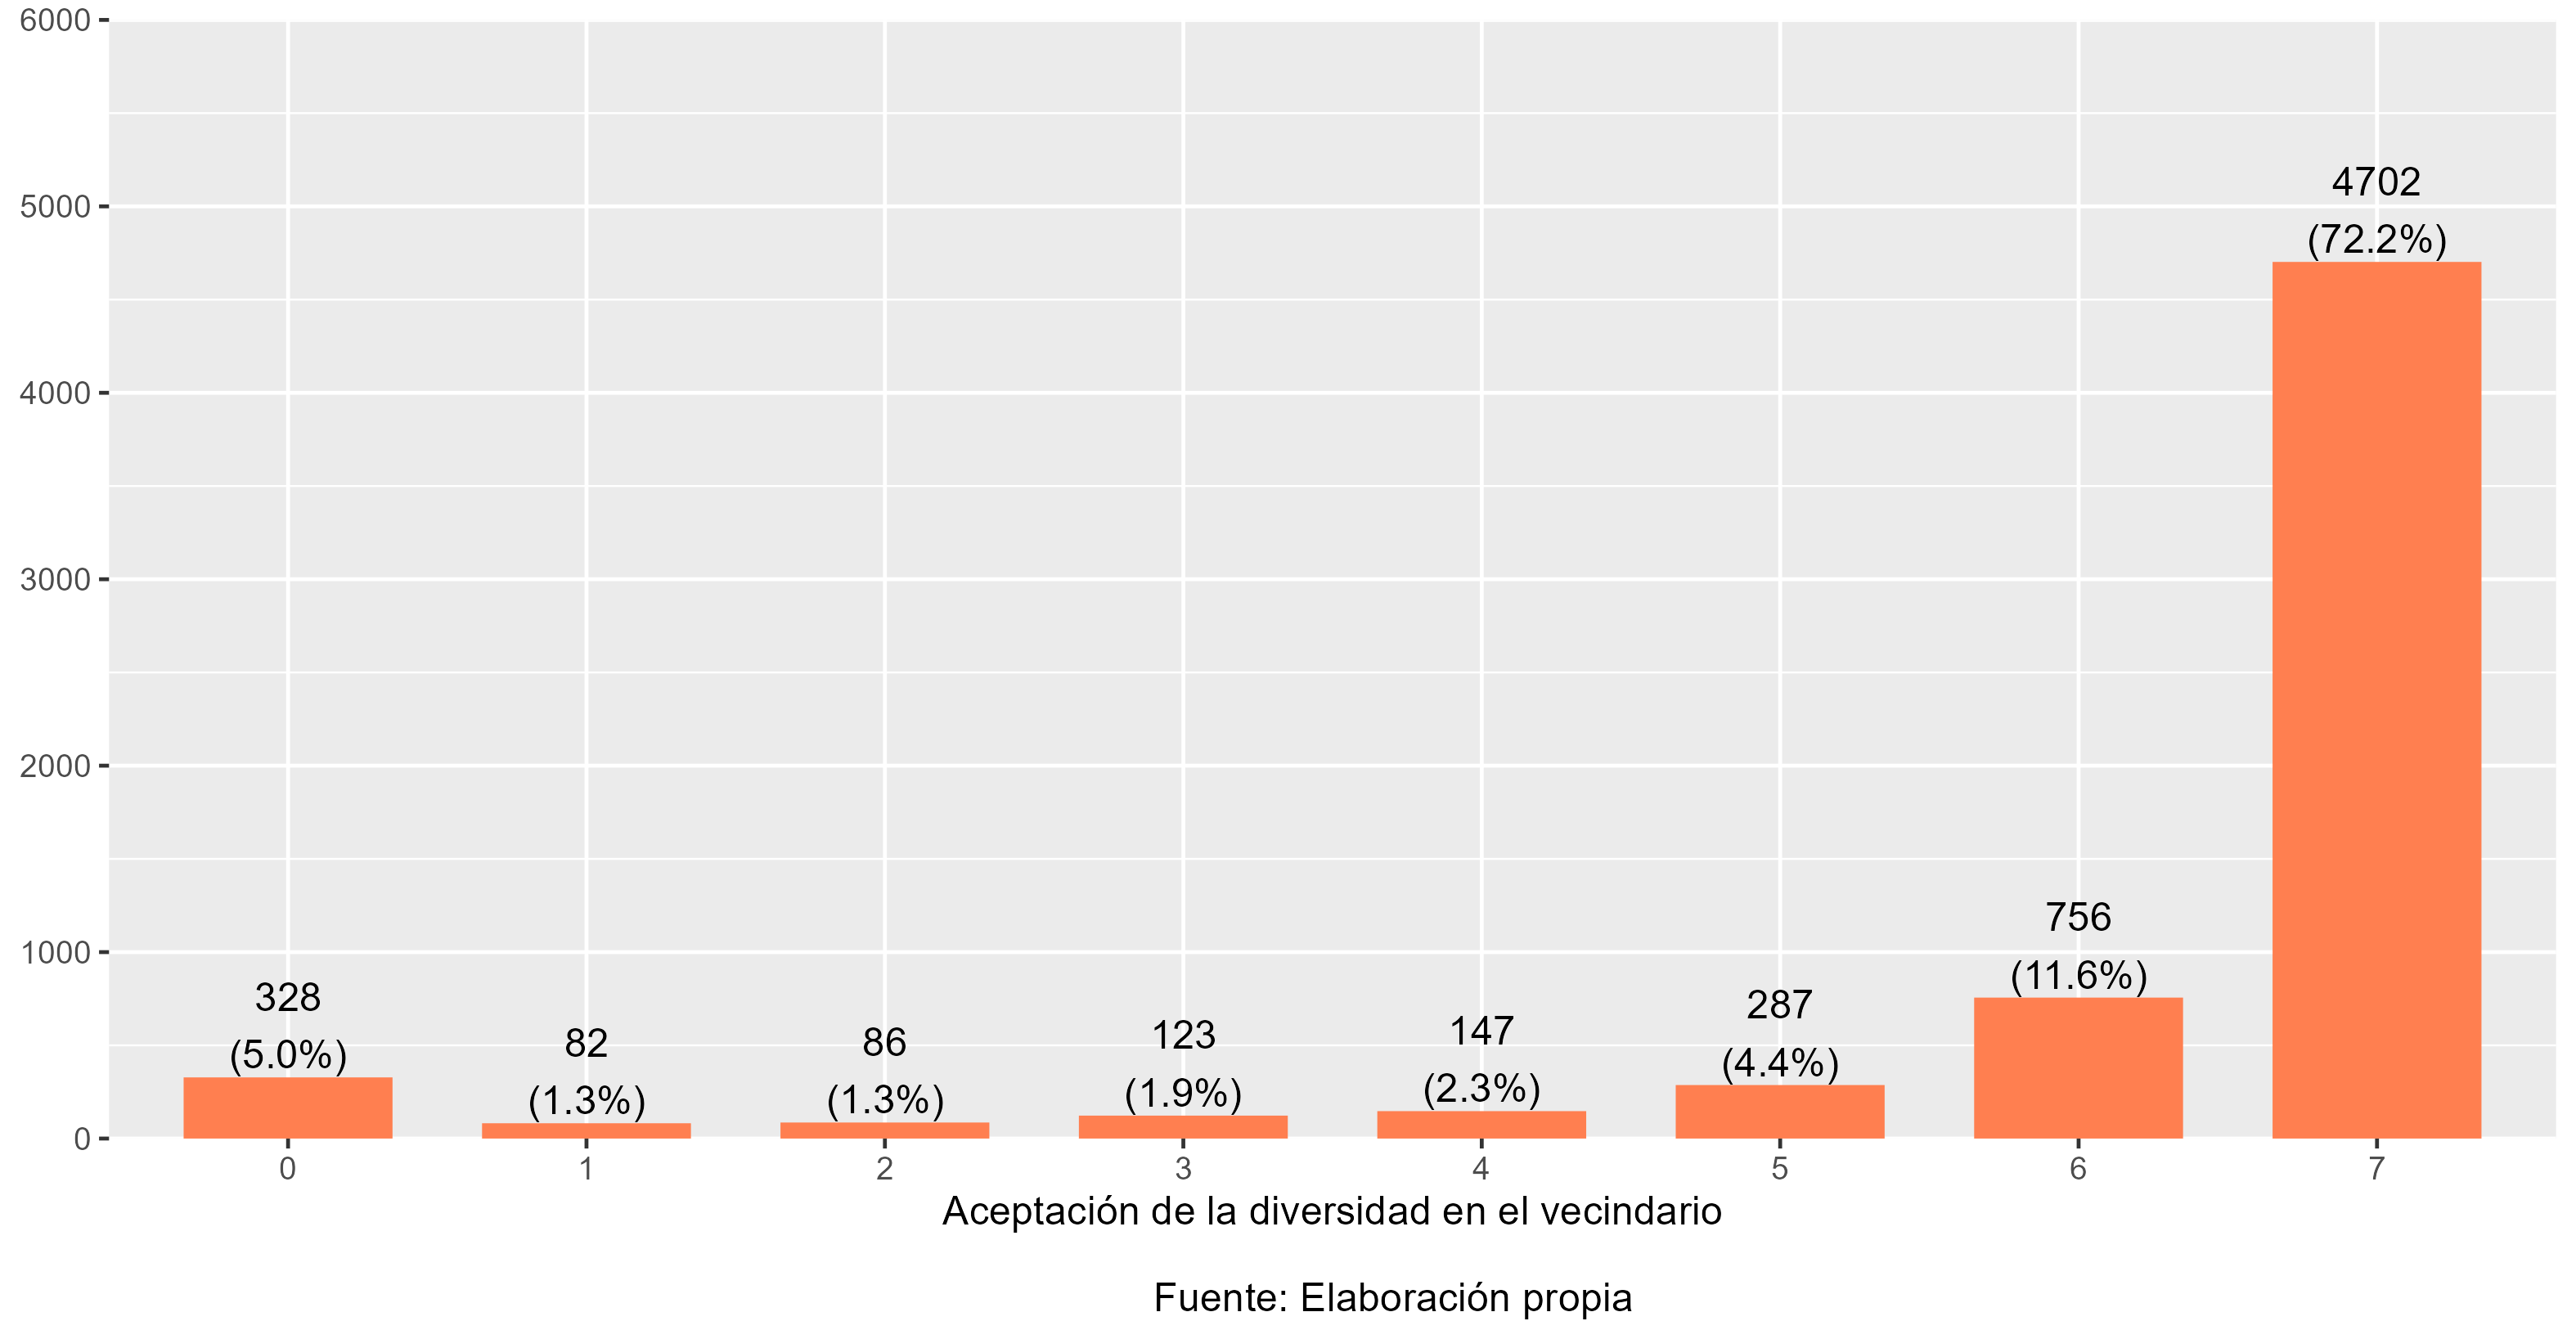
\includegraphics[width=0.8\linewidth,]{IPO/output/graphs/ind_est} 

}

\caption{Indice aceptacion de la diversidad (estudiantes)}\label{fig:ind-est}
\end{figure}

En relación con las variables independientes, estas se dividen en tres grupos: 1) variables de la familia, 2) variables de la escuela y 3) variables del territorio.

\begin{enumerate}
\def\labelenumi{\arabic{enumi})}
\tightlist
\item
  Variables de la familia:
\end{enumerate}

Los recursos socioeconómicos son representados a partir de dos variables:

\begin{itemize}
\item
  Nivel educacional (Nivel más alto entre respondente y Cónyuge/pareja): Esta variable es reportada por apoderados. Es categórica y se representa en una escala de 1 a 10, siendo 10 el nivel educacional más alto posible.
\item
  Cantidad de libros en el hogar: Variable categórica que identifica la cantidad de libros en el hogar según el estudiante. Las categorías de respuesta son: 1) 0 a 10 libros; 2) 11 a 25 libros; 3) 26 a 100 libros; 4) 101 a 200 libros; y 5) 200 o más libros.
\end{itemize}

Actitudes de la familia:

\begin{itemize}
\tightlist
\item
  Aceptación de la diversidad de apoderados: se construye de la misma forma en que se operacionalizará la variable dependiente.
\end{itemize}

\begin{enumerate}
\def\labelenumi{\arabic{enumi})}
\setcounter{enumi}{1}
\tightlist
\item
  Variables de la escuela
\end{enumerate}

\begin{itemize}
\item
  Conocimiento cívico: variable obtenida a partir de la prueba de conocimiento cívico aplicada a los y las estudiantes. La clasificación utilizada se basa en las categorías de ICCS 2016 \citep{agenciacalidaddelaeducacion_informe_2018}, donde Bajo nivel D corresponde a bajo 311 puntos, Nivel D es entre 311 y 394 puntos, Nivel C es entre 395 y 478 puntos, Nivel B es entre 479 y 562 puntos y Nivel A es sobre 562 puntos.
\item
  Percepción de apertura a la discusión en la sala de clases: Esta variable refiere a la percepción de los y las estudiantes sobre los espacios e instancias disponibles en la sala de clases para discutir y opinar sobre diversos temas de interés general. Se realizó un Análisis Factorial Exploratorio que permitió estimar puntajes factoriales a partir de 5 de los 6 ítems disponibles en la base de datos (Para más detalles ver la Tabla \ref{tab:anexo1} del Anexo 1)
\item
  Promedio de percepción de apertura a la discusión en la sala de clases: Variable construída a partir del promedio de percepción de apertura a la discusión en cada escuela. Esto permite identificar los espacios e instancias disponibles en la sala de clases para discutir y opinar sobre diversos temas de interés general a nivel de escuela.
\end{itemize}

\begin{enumerate}
\def\labelenumi{\arabic{enumi})}
\setcounter{enumi}{2}
\tightlist
\item
  Variables del territorio
\end{enumerate}

\begin{itemize}
\item
  Proporción de personas que se identifica con alguna etnia: Proporción de personas de la comuna que se identifica con pueblos originarios según el Censo 2017. Variable categórica agrupada en Bajo, Medio y Alto.
\item
  Proporción de población migrante: Proporción de inmigrantes en la comuna, a partir de datos del Censo 2017. Variable categórica agrupada en Bajo, Medio y Alto
\item
  Promedio de escolaridad: Escolaridad promedio de la comuna, según datos del Censo 2017. Esta variable posee un rango de 6.9 a 11.2.
\end{itemize}

Un resumen de estas variables se presenta en la Tabla \ref{tab:desc02}.

\begin{longtable}[]{@{}l@{}}
\caption{\label{tab:desc02}Descripción variables independientes}\tabularnewline
\toprule()
\endhead
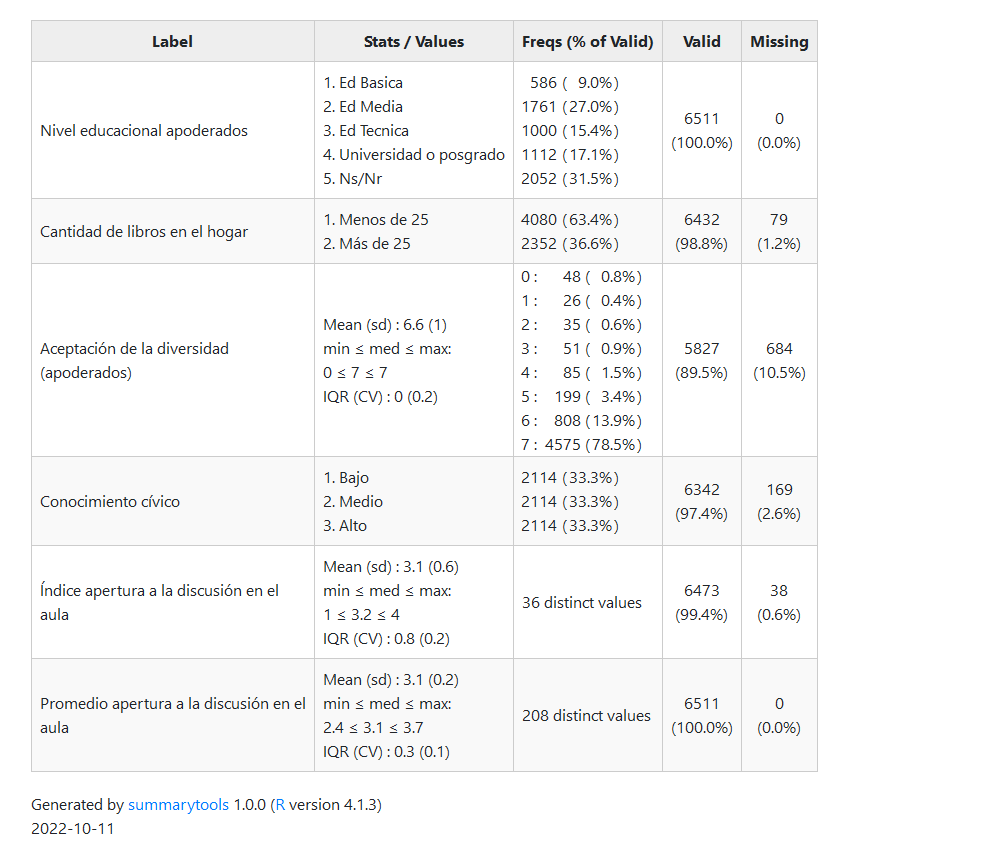
\includegraphics{IPO/output/tables/desc02.png} \\
\bottomrule()
\end{longtable}

\hypertarget{estrategia-de-anuxe1lisis}{%
\section{Estrategia de análisis}\label{estrategia-de-anuxe1lisis}}

La metodología planteada para realizar esta investigación es de carácter cuantitativa. Las hipótesis de esta investigación fueron pre registradas en la plataforma Open Science Framework del Centro de Ciencia Abierta (OSF, Center for Open Science), puede acceder al documento en este \href{https://doi.org/10.17605/OSF.IO/URPZQ}{enlace}. El análisis estadístico de esta investigación fue realizado mediante el software libre R versión 4.0.0.

Debido a que la muestra posee una estructura jerárquica de estudiantes anidados en comunas, se estimarán regresiones multinivel para evaluar todas las hipótesis. Reconocer que se trata de estudiantes anidados en comunas permite incluir variables medidas en diferentes niveles de análisis \citep{aguinis_BestPractice_2013}. Asimismo, realizar una regresión multinivel permite aislar los efectos individuales (estudiantes) de los agregados (comunas) y, a partir de esto, analizar la varianza de los resultados en cada nivel, así como la proporción de la varianza explicada por las variables independientes de cada nivel. Debido a que las características estructurales de los grupos son una dimensión clave para explicar los diferentes resultados que poseen los estudiantes \citep{trevino_Influence_2018} y porque tanto las comunas como las escuelas pueden diferir entre sí en cuanto a sus valores y normas comunes \citep{bayramozdemir_How_2020}, se hace necesario estimar regresiones multinivel que permitan determinar si los resultados en las actitudes de los estudiantes dependen de sus respuestas a nivel individual o por características agregadas a nivel de comuna.

Conceptualmente, existen razones teóricas para esperar encontrar efectos de interacción entre niveles, por lo que también se evaluaran modelos de análisis de moderación, para así determinar si el tamaño o dirección del efecto de las variables independientes sobre la dependiente dependen de algún modo de una tercera variable \citep{hayes_introduction_2022}

De esta forma, luego de estimar la correlación intra-clase de los modelos, y siguiendo los pasos recomendados por \citet{aguinis_BestPractice_2013}, se establecen 3 tipos generales de hipótesis a evaluar:

\begin{itemize}
\item
  Hipótesis de efectos directos a nivel individual (1, 2, 3 y 4)
\item
  Hipótesis de moderación (5)
\item
  Hipótesis de efectos directos a nivel agregado (6, 7 y 8)
\end{itemize}

\hypertarget{resultados}{%
\chapter{Resultados}\label{resultados}}

Se estimó un modelo de regresión multinivel para predecir el índice de aceptación de la diversidad de estudiantes. El modelo incluyó las escuelas (MRBD) como efecto aleatorio. La correlación intra-clase del modelo sin predictores es de 0.012 y el poder explicativo del modelo 4 es débil (R2=0.03). Los resultados de esta estimación se muestran en la Tabla \ref{tab:multinivel}.

\begin{longtable}[]{@{}l@{}}
\caption{\label{tab:multinivel}Regresión multinivel}\tabularnewline
\toprule()
\endhead
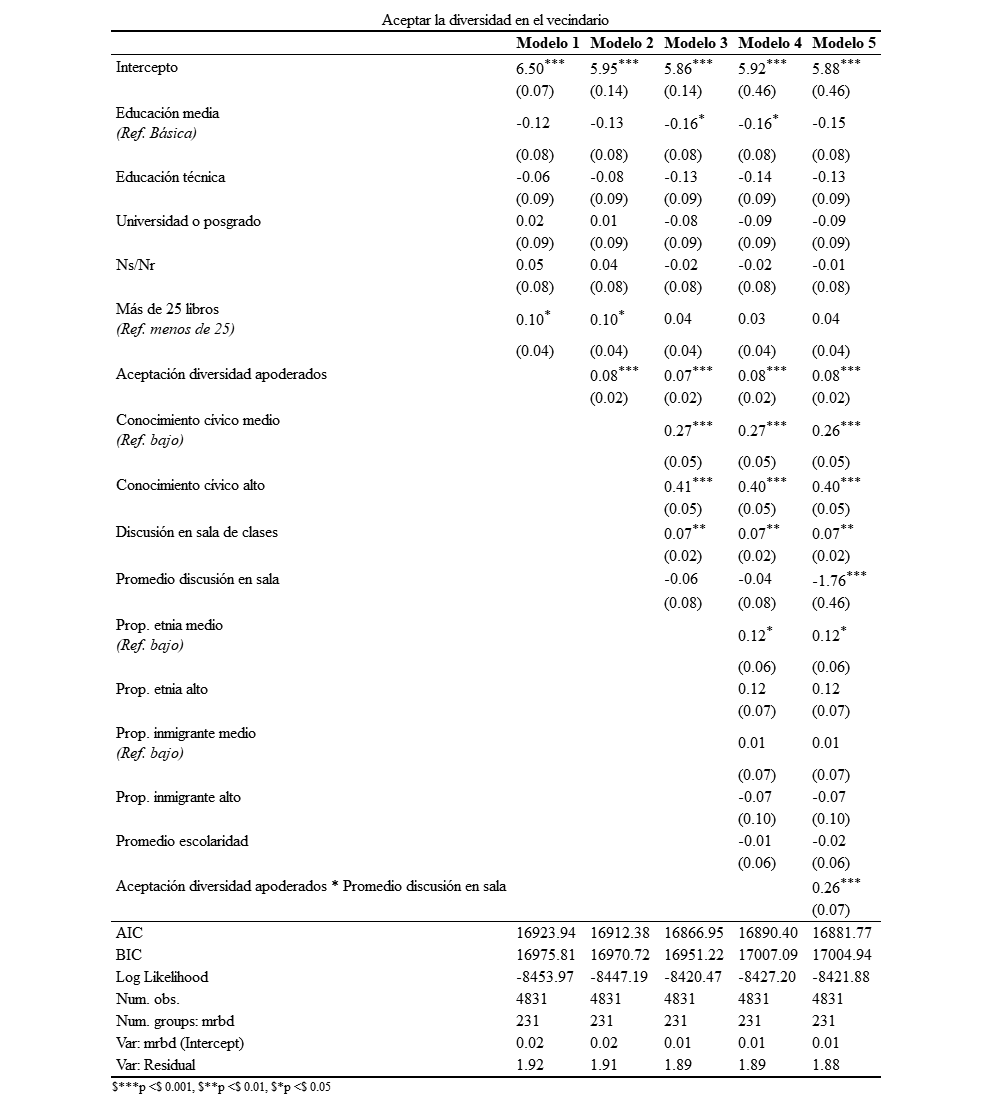
\includegraphics{IPO/output/tables/reg.png} \\
\bottomrule()
\end{longtable}

Las variables asociadas a el nivel educacional de los apoderados no son estadísticamente significativas, salvo para el nivel de educación media en el modelo 3 y 4 (\(\beta\)=-0.16, p \textless{} .05). En cuanto a la cantidad de libros, tener más de 25 libros en el hogar tiene un efecto significativo solo en los modelos 1 y 2 (\(\beta\)=.1, p \textless{} .05), mientras que en el resto de los modelos deja de ser estadísticamente significativa al controlar por las demás variables.

Las actitudes de los apoderados medidas a través del índice de aceptación de la diversidad son estadísticamente significativa al controlar por el resto de las variables y esta relación es consistente en los cuatro modelos en que se incluye esta variable (Modelo 2 y 5 \(\beta\)=.08, p \textless{} .001; Modelo 3 y 4 \(\beta\)=.07, p \textless{} .001).

Las variables asociadas al proceso de socialización en la escuela son estadísticamente significativas en su nivel individual. Tener un nivel de conocimiento cívico C (\(\beta\)=.36, p \textless{} .001), B (\(\beta\)=.54, p \textless{} .001) y A (\(\beta\)=.62, p \textless{} .001) se asocia con una mayor aceptación de la diversidad de los estudiantes en comparación con quienes tienen un nivel de conocimiento cívico bajo el nivel D, al mantener el resto de las variables constantes. El índice de percepción de apertura a la discusión en la sala de clases también se asocia positivamente con la aceptación de la diversidad de los estudiantes (\(\beta\)=.07, p \textless{} .01), manteniendo las demás variables constantes. El promedio de percepción de apertura a la discusión en la sala de clases a nivel de escuela posee una asociación estadísticamente significativa solo en el Modelo 5 al controlar por la moderación entre esta variable y las actitudes de los apoderados (\(\beta\)=-1.76, p \textless{} .001).

Las variables territoriales que abordaban características contextuales de la comuna (proporción de personas que se identifican con alguna etnia, proporción de inmigrantes y promedio de escolaridad) no tienen una asociación estadísticamente significativa con las actitudes de los y las estudiantes.

Finalmente, se estimaron efectos de interacción entre niveles. Estos efectos permiten evaluar si las características contextuales (promedio de percepción de apertura a la discusión en la sala de clases; para el efecto del conocimiento cívico ver la Tabla \ref{tab:interact} del Anexo 2) modifican (moderan) los efectos de las actitudes de los apoderados. En el modelo 5 se muestra que existe una interacción positiva (\(\beta\)=.26, p \textless{} .001) entre el promedio de percepción de apertura a la discusión en la sala de clases y las actitudes de los apoderados.

\begin{figure}[!ht]

{\centering 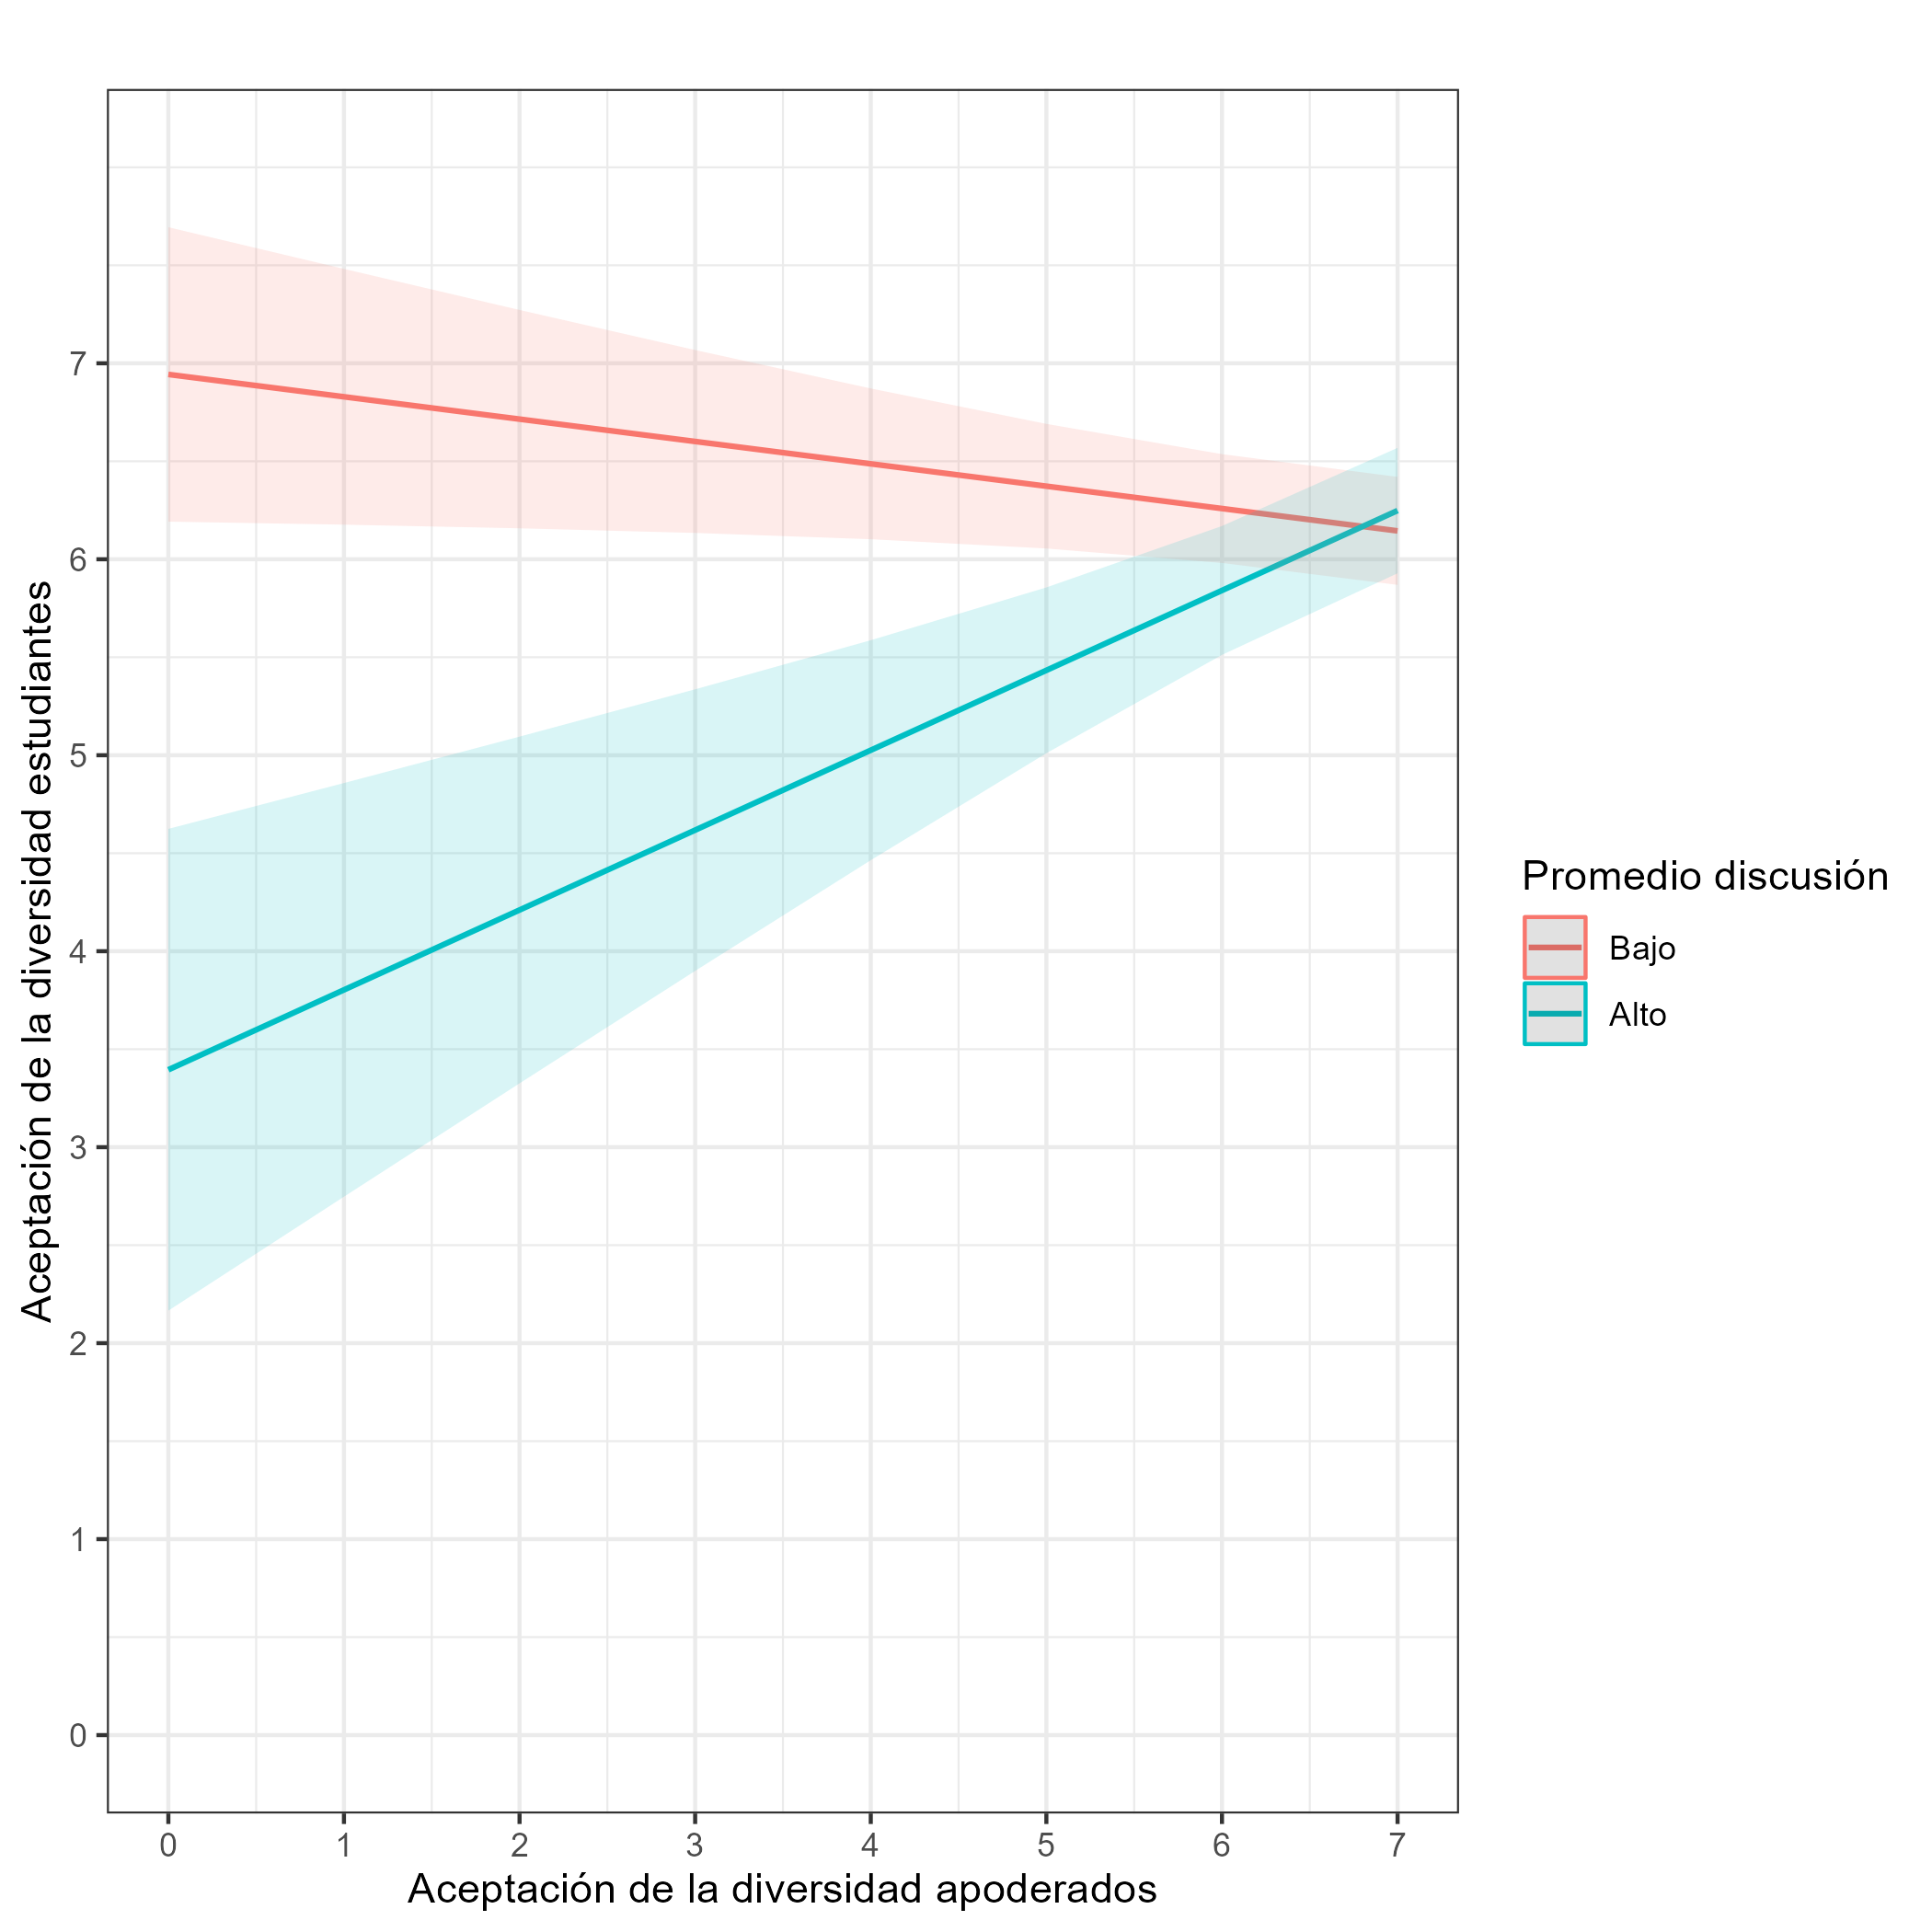
\includegraphics[width=1\linewidth,]{IPO/output/graphs/interac} 

}

\caption{Relación entre actitudes de estudiantes y apoderados moderada por promedio de percepción de apertura a la discusión en la sala de clases}\label{fig:graph-interact}
\end{figure}

El Gráfico \ref{fig:graph-interact} muestra el efecto de la relación entre las actitudes de los estudiantes y sus apoderados, moderada por el promedio de percepción de apertura a la discusión en la sala de clases a nivel de escuela. Esta relación indica que en aquellas escuelas donde exista una baja percepción de apertura a la discusión, la relación entre las actitudes de los estudiantes y apoderados es negativa, mientras que en aquellas escuelas donde existe una alta percepción de apertura a la discusión en la sala de clases las actitudes de los estudiantes se asocian positivamente con las actitudes de los apoderados.

\hypertarget{discusiuxf3n}{%
\chapter{Discusión}\label{discusiuxf3n}}

Los resultados son consistentes con algunas de las hipótesis planteadas. En primer lugar, en cuanto al proceso de socialización familiar, los resultados no permiten comprobar la hipótesis 1 sobre la relación entre los recursos socioeconómicos de la familia y un mayor grado de aceptación de la diversidad en su vecindario. Por el contrario, el único resultado que posee una asociación estadísticamente significativa indica que estudiantes que poseen apoderados con un nivel de educación media aceptarían menos la diversidad en su vecindario en comparación con aquellos estudiantes que poseen apoderados con educación básica. En relación con las actitudes de los apoderados los resultados permiten corroborar la hipótesis planteada (H2), es decir, aquellos estudiantes que provienen de familias con padres que aceptan en mayor medida que distintos grupos sociales vivan en sus vecindarios, también poseen un mayor grado de aceptación de la diversidad en sus vecindarios.

En segundo lugar, los resultados permiten comprobar las hipótesis relacionadas con el proceso de socialización escolar. Estudiantes que poseen un nivel de conocimiento cívico medio y alto poseen un mayor grado de aceptación de la diversidad en sus vecindarios en comparación con estudiantes que poseen un nivel de conocimiento cívico bajo; esto es consistente con la hipótesis 3. En relación con el índice de apertura a la discusión en las salas de clases, los resultados indican que estudiantes que perciben en mayor medida un ambiente abierto a la discusión y al debate dentro del aula poseen un mayor grado de aceptación de la diversidad, lo que permite sustentar la hipótesis 4. En relación con la hipótesis 5 (si la escuela puede mitigar o potenciar el proceso de socialización familiar) los resultados indican que solo el índice de percepción de apertura a la discusión en las salas de clases influyen en la asociación entre actitudes de apoderados y estudiantes.

En tercer lugar, los resultados de las estimaciones de los modelos multinivel no permiten comprobar las hipótesis planteadas que se relacionan con las características de las comunas en que residen los estudiantes, ya que la proporción de personas que se identifican con alguna etnia (H6), la proporción de inmigrantes (H7) y el promedio de escolaridad de la comuna (H8) no influyen en el proceso de socialización de actitudes de los y las estudiantes.

\hypertarget{conclusiones}{%
\chapter{Conclusiones}\label{conclusiones}}

Esta investigación tenía por objetivo evaluar en qué medida los procesos de socialización influyen en las actitudes hacia la diversidad social de estudiantes chilenos. En concreto, se evaluó si los procesos de socialización familiar y escolar, además de algunas características territoriales, podían influir en las actitudes de los estudiantes. En términos generales los resultados permiten identificar el rol de la transmisión intergeneracional de actitudes dentro del proceso de socialización familiar y el rol del conocimiento cívico y la percepción de apertura a la discusión en el aula dentro del proceso de socialización escolar.

De acuerdo con la literatura las características socioeconómicas de las familias poseen un rol preponderante en el proceso de formación de los estudiantes, sin embargo, los resultados no van en línea con este supuesto, sino que son las actitudes de los apoderados los que influyen en las actitudes de los estudiantes.

En cuanto al proceso de socialización escolar, el nivel de conocimiento cívico y la percepción de apertura a la discusión en el aula influyen en las actitudes de los estudiantes, pero solo en las escuelas con una mayor percepción de apertura a la discusión se logra potenciar la relación entre las actitudes de los apoderados y los estudiantes. Esto indica a grandes rasgos que si las actitudes cívicas no se practican todos los días, insistiendo solo en el currículo escolar y dejando fuera los espacios cotidianos de convivencia de los y las estudiantes, se corre el riesgo de generar conocimientos lejanos a la experiencia real de los estudiantes.

Una de las principales limitaciones de este estudio es la poca varianza que tienen las variables de tolerancia a cada uno de los grupos estudiados (antes de la construcción del índice) y que imposibilitan realizar un análisis más preciso de la dimensionalidad de la variable dependiente. Asimismo, no poseer datos de identificación de los vecindarios o unidades censales en que viven los estudiantes limita los resultados, ya que es posible que el nulo efecto de las variables territoriales se deba a que corresponden a agrupaciones comunales que no permiten medir el efecto real del contexto en que viven los estudiantes.

Finalmente, así como la discusión y el debate escolar influyen en las actitudes de los estudiantes, sería interesante problematizar e investigar si la participación en espacios extra-escolares, de los vecindarios y territorios, puede influir en la tolerancia y aceptación de la diversidad. Traspasar la Escuela como único formador de ciudadanos y conocer qué otros factores puedan influir en la socialización de actitudes es una agenda de investigación futura.

En resumen, los resultados proveen evidencia adicional de acuerdo con factores y condiciones que tienen el potencial de ayudar a las escuelas y profesores a promover la tolerancia. Por lo tanto, las escuelas continúan teniendo un rol fundamental en el proceso de socialización de las nuevas generaciones y, en definitiva, el foco debe estar en que estos mecanismos sean transversales a todo el sistema educacional.

\hypertarget{anexos}{%
\chapter{Anexos}\label{anexos}}

\hypertarget{anexo-1}{%
\subsection{Anexo 1}\label{anexo-1}}

\begin{longtable}[]{@{}l@{}}
\caption{\label{tab:anexo1}Análisis factorial exploratorio}\tabularnewline
\toprule()
\endhead
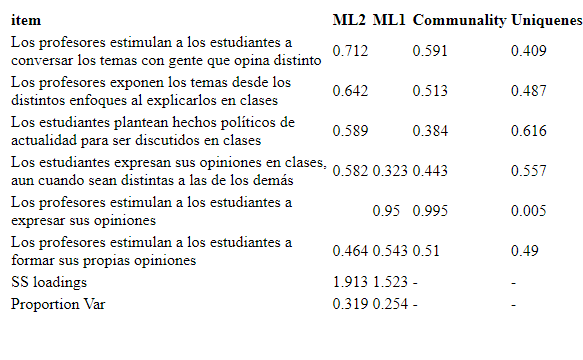
\includegraphics{IPO/output/tables/apdis_fa.png} \\
\bottomrule()
\end{longtable}

\hypertarget{anexo-2}{%
\subsection{Anexo 2}\label{anexo-2}}

\begin{longtable}[]{@{}l@{}}
\caption{\label{tab:interact}Interacciones entre niveles}\tabularnewline
\toprule()
\endhead
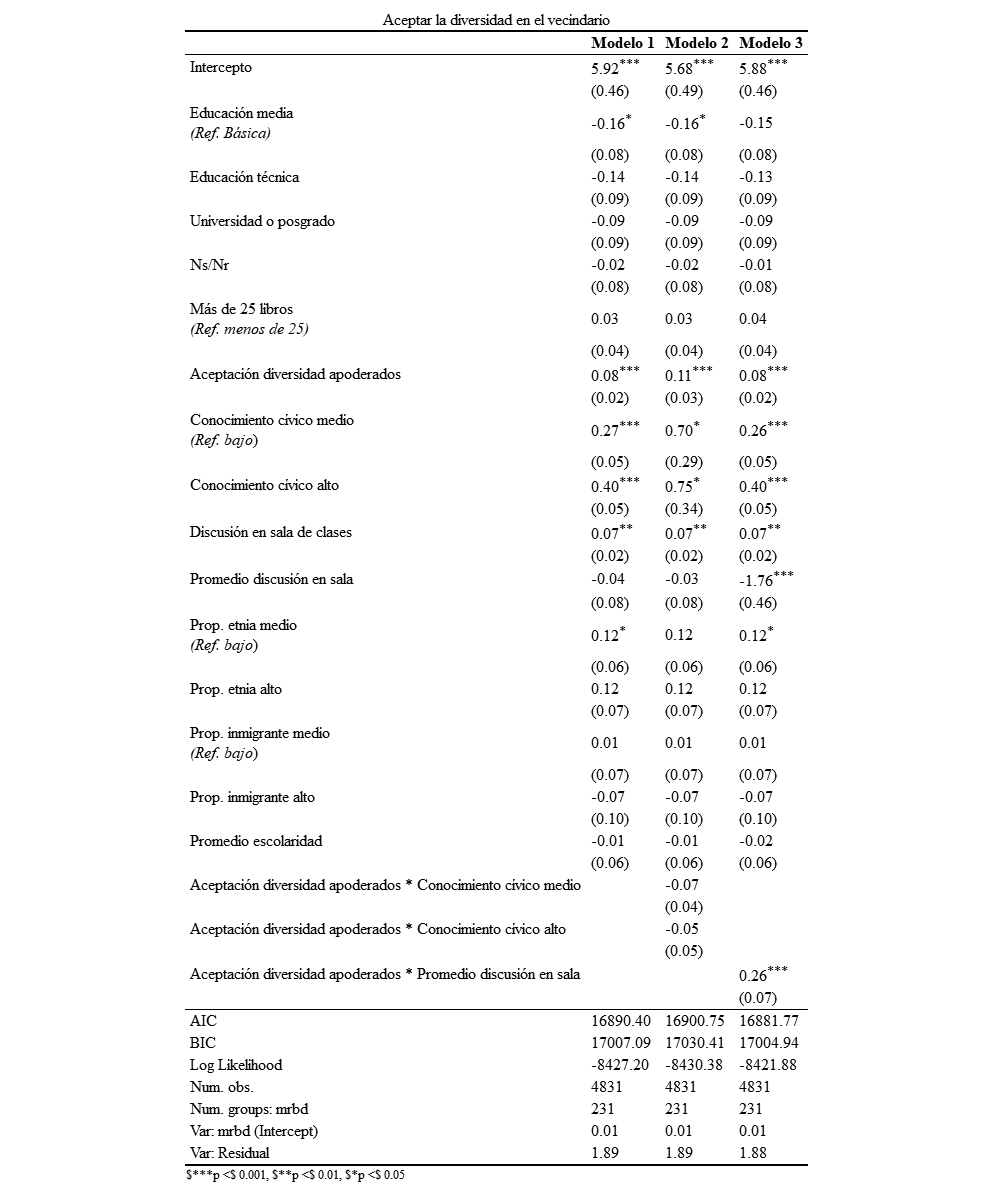
\includegraphics{IPO/output/tables/interac.png} \\
\bottomrule()
\end{longtable}

\hypertarget{bibliografuxeda}{%
\chapter*{Bibliografía}\label{bibliografuxeda}}
\addcontentsline{toc}{chapter}{Bibliografía}

% %%%%%%%%%%%%%%%%%%%%%%%%%%%%%%%%%%%%%%%%%%%%%%%%%
% %%% Bibliography                              %%%
% %%%%%%%%%%%%%%%%%%%%%%%%%%%%%%%%%%%%%%%%%%%%%%%%%
% \addtocontents{toc}{\vspace{.5\baselineskip}}
% \cleardoublepage
% \phantomsection
% \addcontentsline{toc}{chapter}{\protect\numberline{}{Bibliography}}
\bibliography{tesis}

%% All books from our library (SfS) are already in a BiBTeX file
%% (Assbib). You can use Assbib combined with your personal BiBTeX file:
%% \bibliography{Myreferences,Assbib}. Of course, this will only work on
%% the computers at SfS, unless you copy the Assbib file
%%  --> /u/sfs/bib/Assbib.bib



\end{document}
